\chapter{MARCO TEÓRICO}
\label{cap:teorico}

El reconocimiento de elementos arquitectónicos en nubes de puntos del patrimonio
construido es un tema interdisciplinario, que reúne la ingeniería civil y la
computación. Este marco teórico define los conceptos que sustentan el diseño de la
tesis (Figura~\ref{fig:diseno}): los del objeto de estudio, los de computación y
los algoritmos, y las métricas con que se evalúa el modelo.

% =====================================================================
\section{Ingeniería Civil y Conservación del Patrimonio}
\label{sec:civil}

La ingeniería civil es clave para la conservación del patrimonio
arquitectónico, ya que proporciona las herramientas necesarias para la
documentación, el análisis y la preservación de estructuras históricas como la
Catedral de Lima. A continuación se presentan los conceptos fundamentales de
esta disciplina que son relevantes para este trabajo, desde la nube de puntos y
el levantamiento que la produce hasta su preparación y su segmentación.

\subsection{Nube de Puntos y su Captura}
\label{sec:nube}

Una nube de puntos es un conjunto $P=\{(x_i,f_i)\}_{i=1}^{N}$ donde
\nom{xi}{$x_i\in\mathbb{R}^3$} es la posición medida de un punto de la superficie y $f_i$
sus atributos. No tiene conectividad ni orden. Es una lista de mediciones, no
una malla.
Se almacena como una tabla con una fila por punto y una
columna por valor. En este trabajo los atributos son el color, que registra el
sensor, y la normal, que se estima a partir de los vecinos.
Es el dato de entrada y el objeto que se segmenta.

\paragraph*{Levantamiento Láser Terrestre (TLS)}\phantomsection
\label{sec:tls}

Registra una edificación con un escáner estacionado en posiciones fijas, que emite
un haz y calcula la posición de cada punto a partir de la distancia y la dirección
del retorno. Es la técnica con que se levantó la Catedral de Lima.

\paragraph*{Formato LAS}\phantomsection
\label{sec:las}

Es el formato estándar de la ASPRS para intercambiar nubes de puntos láser. Cada
registro de punto guarda las coordenadas, más atributos como la intensidad del
retorno, la clase y, según el formato, el color RGB.

\subsection{Centrado de Coordenadas}
\label{sec:centrado}

El centrado traslada la nube al origen restándole el centro de su caja envolvente:
\begin{equation}
\nom{c}{c}=\tfrac{1}{2}\left(\nom{minmax}{\min}_i \nom{xi}{x_i}+\nom{minmax}{\max}_i \nom{xi}{x_i}\right),\qquad \nom{xip}{x_i'}=\nom{xi}{x_i}-\nom{c}{c} ,
\label{eq:centrado}
\end{equation}
El vector \nom{c}{$c$} se guarda para revertir el centrado.

Las coordenadas del levantamiento son números muy grandes: en el eje norte superan
los 8 millones de metros. En precisión simple, que guarda unos siete dígitos, a esa
magnitud dos valores consecutivos están a un metro, y puntos separados por
centímetros quedarían iguales. Restar el centro reduce las coordenadas a decenas de
metros y conserva ese detalle.

\subsection{Vecindad de los $q$ Vecinos y Filtrado de Valores Atípicos (SOR)}
\label{sec:knn}

La vecindad (KNN) de un punto $i$ es el conjunto \nom{vec}{$\mathcal{N}_q(i)$} de los
\nom{q}{$q$} puntos más próximos a él en distancia euclídea; en este trabajo,
$q=20$. La nube se indexa en un árbol $k$-d, que divide el espacio de forma
recursiva y evita comparar cada punto con todos los demás.

\paragraph*{Filtrado Estadístico de Valores Atípicos (SOR)}\phantomsection
\label{sec:sor}

Descarta los puntos aislados, como reflejos en vidrios o personas que cruzaron
durante el escaneo. Para cada punto se mide su distancia media a los $q$ vecinos
más cercanos, \nom{dbar}{$\bar d_i$}; el promedio $\mu$ y la desviación estándar
$\sigma$ de esas distancias dicen cuál es la distancia normal entre vecinos. Se
conserva el punto si no está más lejos que lo normal más $\lambda$ desviaciones:
\begin{equation}
\nom{dbar}{\bar d_i}\le\nom{musigma}{\mu}+\nom{lam}{\lambda}\,\nom{musigma}{\sigma} ,
\label{eq:sor}
\end{equation}
\noindent Un $\lambda$ menor descarta más puntos pero puede borrar detalle fino; se
usa $\lambda=2$. Limpia la nube antes de voxelizarla, para que los puntos
espurios no se promedien con los válidos.

\subsection{Vóxel y Voxelización}
\label{sec:voxel}

Un vóxel es una celda cúbica de una rejilla regular que divide el espacio; su lado
es el tamaño de vóxel. La voxelización sustituye los puntos de cada vóxel $v$ por
un único representante, cuya posición y color son el promedio de los del grupo:
\begin{equation}
\nom{xv}{\bar x_v}=\frac{1}{\nom{xv}{|v|}}\nomop{suma}{\sum}_{i\in \nom{xv}{v}}\nom{xi}{x_i} ,
\label{eq:voxel}
\end{equation}
Reduce los registros y homogeniza la densidad, que en un levantamiento láser es
muy alta cerca del escáner y baja lejos de él. No es un paso de limpieza:
conserva todas las superficies y solo reduce los registros que las describen. Se
usa un vóxel de 5\,cm.

\subsection{Normal de Superficie y su Estimación}
\label{sec:normales}

La normal de un punto es el vector unitario
\nom{n}{$n_i=(n_x,n_y,n_z)$} perpendicular a la superficie en ese punto; dice
hacia dónde mira la superficie. El escáner no la mide, así que se estima con la
matriz de covarianza de los $q$ vecinos más cercanos del punto,
\nom{pbar}{$p_1,\ldots,p_q$}, cuyo promedio es el centroide
\nom{pbar}{$\bar p$}:
\begin{equation}
\nom{cov}{C}=\frac{1}{\nom{q}{q}}\nomop{suma}{\sum}_{j=1}^{q}\left(\nom{pbar}{p_j}-\nom{pbar}{\bar p}\right)\left(\nom{pbar}{p_j}-\nom{pbar}{\bar p}\right)^{\nom{T}{\top}}.
\label{eq:normal}
\end{equation}
\noindent Sus tres autovectores son las direcciones principales de dispersión,
cada una con un autovalor que mide cuánto se dispersan los vecinos a lo largo de
ella. Sobre una superficie, la dirección de menor variación es aproximadamente la
perpendicular: la normal es el autovector de \nom{cov}{$C$} con el menor
autovalor.

\subsection{Sección Espacial}
\label{sec:seccion}

Una sección es la porción del levantamiento que se preprocesa en una misma
corrida: reúne uno o varios archivos LAS, o un solo escaneo si hay un archivo por
corrida. Su salida \nom{S}{$S$} es una matriz de \nom{N}{$N$} filas, una por punto,
y nueve columnas en precisión simple,
\begin{equation}
\nom{S}{S}=\left[\,\nom{xyz}{x\;\;y\;\;z}\;\;\nom{rgb}{R\;\;G\;\;B}\;\;\nom{n}{n_x\;\;n_y\;\;n_z}\,\right],
\label{eq:sj}
\end{equation}
De cada punto del LAS se conservan la posición $(x,y,z)$, que se centra, y el color
$(R,G,B)$, llevado de 16~bits al rango 0 a 255; la normal se estima y queda
unitaria. Como el autovector no fija el sentido de la normal, la implementación invierte las que apuntan hacia abajo
para que todas cumplan $n_z\geq 0$; así no distingue la cara interior de un muro
de la exterior.

\subsection{Segmentación Semántica y Clases}
\label{sec:segsem}

La segmentación semántica asigna una etiqueta de clase a cada punto de $P$. Se
distingue de la segmentación de instancias, que además separa objetos distintos
de una misma clase y queda fuera del alcance de este trabajo.

\paragraph*{Clase Conocida y Clase Novedosa}\phantomsection
\label{sec:clases}

\nom{Ck}{$\mathcal{C}_k$} es el subconjunto de clases con puntos etiquetados durante el
entrenamiento y \nom{Cn}{$\mathcal{C}_n$} el de clases presentes en la nube pero sin
ninguna etiqueta, con $\mathcal{C}_k\cap\mathcal{C}_n=\emptyset$ y
$\mathcal{C}=\mathcal{C}_k\cup\mathcal{C}_n$. En patrimonio, $\mathcal{C}_n$
recoge los elementos singulares de cada edificio, que no figuran en ningún
catálogo previo. 

% =====================================================================
\section{Computación}
\label{sec:computacion}

\subsection{Descriptor de Punto}
\label{sec:descriptor}
\label{sec:concat}

Un descriptor es el vector numérico que resume el contenido de un punto o de una
región. HyperNCD~\cite{zhang2026hyperncd} describe cada punto concatenando dos
componentes:
\begin{equation}
\nom{Fi}{F_i}=\left[\nom{fsem}{f_{\mathrm{sem}}}(\nom{xi}{x^i})\nom{concat}{;}\,\nom{fgeo}{f_{\mathrm{geo}}}(\nom{xi}{x^i})\right].
\label{eq:hyperncd3}
\end{equation}
Este trabajo sustituye el segundo componente por el descriptor
auto-supervisado:
\begin{equation}
\nom{Fi}{F_i}=\left[\nom{fsem}{f_{\mathrm{sem}}}(\nom{xi}{x^i})\nom{concat}{;}\,\nom{fssl}{f_{\mathrm{ssl}}}(\nom{xi}{x^i})\right].
\label{eq:hibrido}
\end{equation}
El punto y coma indica concatenación: un vector a continuación del otro.

\subsubsection{Descriptor Semántico}
\label{sec:fsem}

Vector que la red troncal supervisada de HyperNCD, una MinkowskiUNet-34C, entrega
por cada punto. Codifica a qué se parece un punto en términos de las clases y
pseudo-etiquetas usadas durante el entrenamiento.

En fórmulas, cada punto cae en una celda de lado $\nom{ell}{\ell}=5$\,cm, cada
vóxel ocupado recibe la característica constante 1 (el color y la normal no
entran) y la red $\nom{Unet}{U_\theta}$ devuelve un vector de 96 canales por
vóxel ocupado:
\begin{equation}
\nom{vcel}{\mathbf{v}_i}=\left\lfloor \frac{\nom{xi}{x_i}}{\nom{ell}{\ell}}\right\rfloor,\qquad a_{\mathbf{v}}=1,
\label{eq:cuant}
\end{equation}
\begin{equation}
\nom{fsem}{f_{\mathrm{sem}}}(\nom{xi}{x^i})=\nom{Unet}{U_\theta}(\mathcal{V})_{\nom{vcel}{\mathbf{v}_i}}\in\mathbb{R}^{96},
\label{eq:fsem}
\end{equation}
donde $\mathcal{V}$ es el tensor disperso formado por las celdas ocupadas y sus
características $a_{\mathbf{v}}$. Los puntos que comparten celda comparten
descriptor.

\subsubsection{Descriptor Geométrico Analítico}
\label{sec:fgeo}

Vector calculado con una fórmula cerrada, sin aprendizaje, a partir de los
autovalores \nom{eig}{$\lambda_1\geq\lambda_2\geq\lambda_3$} de la matriz de
covarianza de un conjunto de puntos: linealidad, planaridad y dispersión. El
artículo los calcula sobre un vecindario de 15 puntos; la implementación
ejecutada los calcula sobre la región que contiene al punto y les concatena el
centroide de esa región, lo que da dimensión 6,
\begin{equation}
\nom{g}{g^{(r)}}=\left[\frac{\nom{eig}{\lambda_1}-\nom{eig}{\lambda_2}}{\nom{eig}{\lambda_1}},\;\frac{\nom{eig}{\lambda_2}-\nom{eig}{\lambda_3}}{\nom{eig}{\lambda_1}},\;\frac{\nom{eig}{\lambda_3}}{\nom{eig}{\lambda_1}},\;c^{(r)}\right]\in\mathbb{R}^{6},
\label{eq:g-region}
\end{equation}
donde los $\lambda$ son los autovalores de la covarianza de los puntos de la
región $r$ y $c^{(r)}$ es su centroide. Este trabajo adopta la versión ejecutada,
en la que cada punto hereda el descriptor de su región. Se denota
$f_{\mathrm{geo}}$ y es el componente que este trabajo sustituye. Solo describe
forma, sin ningún conocimiento de qué es el punto.

\subsubsection{Descriptor Auto-supervisado}
\label{sec:fssl}

Salida del codificador PTv3 preentrenado de Sonata~\cite{wu2025sonata}, usado con
pesos congelados. Su dimensión es 1088. Se denota $f_{\mathrm{ssl}}$ y codifica
estructura aprendida sobre 140 mil escenas, sin haber visto las clases de este
proyecto. A diferencia de $f_{\mathrm{geo}}$, no es un descriptor de forma: el
preentrenamiento de Sonata está diseñado para evitar el atajo geométrico, de modo
que aporta un conocimiento semántico adquirido sin etiquetas, complementario al
supervisado de $f_{\mathrm{sem}}$. Por eso el modelo es híbrido.

\subsection{Aprendizaje Auto-supervisado}
\label{sec:ssl}

Régimen de entrenamiento en el que la señal de supervisión se construye a partir de
los propios datos y no de etiquetas humanas. Es el régimen con que se preentrenó el
codificador de Sonata.

\paragraph*{Codificador Congelado}\phantomsection
\label{sec:congelado}

Red cuyos pesos no se actualizan y que se usa solo en inferencia. Su costo se paga
una sola vez y no en cada época, lo que permite calcular su salida por adelantado
y guardarla en disco.

\paragraph*{Atajo Geométrico}\phantomsection
\label{sec:atajo}

Modo de falla del preentrenamiento auto-supervisado, diagnosticado por Sonata, en
el que la representación colapsa sobre pistas geométricas fácilmente accesibles,
como la normal, la altura o la curvatura local, en lugar de aprender semántica. Es
la razón por la que este trabajo sustituye $f_{\mathrm{geo}}$.

\subsection{Serialización y Codificador PTv3}
\label{sec:serializacion}

Ordenamiento de los puntos mediante una curva de llenado de espacio, de tipo Z o
Hilbert, para que la proximidad en $\mathbb{R}^3$ se traduzca en proximidad dentro
de una secuencia unidimensional. La secuencia se corta en parches contiguos y la
atención se aplica solo dentro de cada uno, lo que da a PTv3~\cite{wu2024ptv3} un
costo lineal.

\paragraph*{Codificador PTv3}\phantomsection
\label{sec:codificador-ptv3}

Es el codificador de Sonata: un PTv3~\cite{wu2024ptv3} que aplica cuatro
operaciones (detalles en el \hyperref[sec:arq-sonata]{Anexo~C}). Primero, un
\emph{embedding} convierte los nueve valores $\nom{xin}{\mathbf{x}_i}$ de cada
punto en un vector de 48 características,
\begin{equation}
\nom{h}{\mathbf{h}_i^{(0)}}=\mathrm{GELU}\!\left(\mathrm{LN}\!\left(\nom{We}{W_e}\,\nom{xin}{\mathbf{x}_i}+\nom{We}{b_e}\right)\right),
\label{eq:embedding}
\end{equation}
donde $W_e$ y $b_e$ son parámetros aprendidos, y LN y GELU, una normalización y
una activación. Segundo, cada bloque combina una convolución dispersa que codifica
la posición, la atención y un MLP. La atención es la de los
Transformers~\cite{vaswani2017attention}, aplicada dentro de cada parche de 1024
puntos, cuyas características reúne $\nom{Hp}{\mathbf{H}_p}$:
\begin{equation}
\mathrm{Atn}(\nom{Hp}{\mathbf{H}_p})=\mathrm{softmax}\!\left(\frac{(\nom{Hp}{\mathbf{H}_p}\nom{WQKV}{W_Q})(\nom{Hp}{\mathbf{H}_p}\nom{WQKV}{W_K})^{\nom{T}{\top}}}{\sqrt{\nom{dcab}{d}}}\right)\nom{Hp}{\mathbf{H}_p}\nom{WQKV}{W_V},
\label{eq:atencion}
\end{equation}
con $W_Q$, $W_K$ y $W_V$ matrices aprendidas y $d$ los canales por cabeza; cada fila
de softmax indica cuánto atiende un punto a los demás del parche. Tercero, entre
etapas el \emph{pooling} duplica el lado de la celda y toma el máximo por celda.
Cuarto, el \emph{up-cast} reúne las tres últimas etapas.

\subsection{Red Dispersa de Minkowski}
\label{sec:rejilla}
\label{sec:tensor}

Una rejilla dispersa es una rejilla de vóxeles de la que solo se almacenan los
ocupados. Un edificio ocupa una fracción mínima del volumen que lo envuelve, así
que guardar también los vóxeles vacíos sería inviable. Un tensor disperso es la
estructura de datos que la representa en MinkowskiEngine: una lista de
coordenadas enteras de vóxel y, por cada una, un vector de características.

\paragraph*{Convolución Dispersa}\phantomsection
\label{sec:convdispersa}

Es la operación definida sobre un tensor disperso.
Como una convolución ordinaria, combina las
características de un vóxel con las de sus vecinos dentro de un núcleo cúbico
mediante pesos aprendidos, pero solo se evalúa en los vóxeles ocupados y solo
considera vecinos ocupados. La vecindad es por tanto métrica: son vecinos los vóxeles adyacentes en el volumen. Es la capa con que está construida la red que produce
$f_{\mathrm{sem}}$, y su noción de vecindad no coincide con la de la
serialización.

\paragraph*{MinkowskiUNet-34C}\phantomsection
\label{sec:minkunet}

Es la red troncal de HyperNCD, una red de convoluciones dispersas
con arquitectura codificador-decodificador.
Tiene tres partes.
\begin{itemize}\setlength{\itemsep}{1pt}
\item \textbf{Codificador} (\emph{encoder}). Cuatro niveles que reducen la
resolución a la mitad cada vez y aumentan el número de canales, con anchuras
$(32,64,128,256)$. Cada nivel ve una porción mayor del edificio con menos
detalle.
\item \textbf{Decodificador} (\emph{decoder}). Cuatro niveles que devuelven la
resolución original, con anchuras $(256,128,96,96)$.
\item \textbf{Conexiones de salto} (\emph{skip connections}). Cada nivel del
decodificador recibe, concatenada, la salida del nivel del codificador que tiene
su misma resolución. Así recupera el detalle fino que el submuestreo perdió.
\end{itemize}

\subsection{Muestreo por Rejilla e Índice Inverso}
\label{sec:gridsample}

El muestreo por rejilla es la discretización que la rutina de preparación de
Sonata aplica a la nube antes del codificador: la divide en celdas de 2\,cm y
conserva un punto por celda ocupada. El índice inverso es la tabla que anota, para
cada punto de la entrada, la celda en la que cayó; con ella, el descriptor de cada
celda vuelve a todos los puntos de $S$ que cayeron en ella, de modo que
$f_{\mathrm{ssl}}$ queda definido sobre los mismos puntos del Módulo~1. Como la
celda es más fina que el vóxel del preprocesamiento, casi todos los puntos quedan
solos en su celda.

\paragraph*{Propagación Inversa del Submuestreo}\phantomsection
\label{sec:upcast}

También llamada \emph{up-cast}, devuelve las características del codificador a la
resolución de entrada reutilizando los índices de agrupamiento que el propio
submuestreo registró. Cada punto $x^i$ de $S$ recibe las características de las
tres últimas etapas en la celda en la que cayó:
\begin{equation}
\nom{fssl}{f_{\mathrm{ssl}}}(\nom{xi}{x^i})=\left[\,\nom{h}{\mathbf{h}^{(3)}}_{\nom{pis}{\pi_3(\nom{inv}{\mathrm{inv}(i)})}}\,;\,\nom{h}{\mathbf{h}^{(4)}}_{\nom{pis}{\pi_4(\mathrm{inv}(i))}}\,;\,\nom{h}{\mathbf{h}^{(5)}}_{\nom{pis}{\pi_5(\mathrm{inv}(i))}}\,\right]\in\mathbb{R}^{192+384+512},
\label{eq:upcast}
\end{equation}
donde $\mathrm{inv}(i)$ es esa celda y $\pi_s(j)$ la celda de la etapa $s$ que
contiene a la celda $j$, obtenida encadenando los índices del submuestreo.

\subsection{Corte de Sección y Reconstrucción de Superficie}
\label{sec:caja}

La caja de sección (\emph{section box}) es un paralelepípedo que se ajusta sobre
la nube para mostrar solo los puntos que quedan dentro; el corte es un plano que
oculta todo lo que queda a un lado. Ambos permiten inspeccionar el interior de
un edificio sin que el resto lo tape. 

\paragraph*{Reconstrucción de Superficie de Poisson}\phantomsection
\label{sec:poisson}

Método que convierte una nube de puntos con normales en una malla cerrada:
busca la superficie cuya orientación mejor coincide con las normales de los
puntos. La malla resultante puede exportarse como sólido en formatos de
modelado 3D como OBJ, PLY o STL.  Se usa para exportar un elemento ya segmentado.

% =====================================================================
\section{Algoritmos}
\label{sec:algoritmos}

Esta sección reúne los procedimientos con que se descubren las clases
novedosas y las arquitecturas de los dos métodos que el trabajo combina.

\subsection{Descubrimiento de Clases Novedosas (NCD)}
\label{sec:ncd}

El NCD consiste en producir una asignación $\hat{y}:P\rightarrow\mathcal{C}$
correcta sobre $\mathcal{C}_k$ y consistente sobre $\mathcal{C}_n$, entendiendo
por consistente que los puntos de una misma clase novedosa reciban la misma
etiqueta, aunque esa etiqueta no tenga nombre. La etiqueta que recibe el punto
$i$ se denota \nom{y}{$\hat{y}_i$}. 

\subsection{Región o Superpunto}
\label{sec:region}

Una región es una agrupación de puntos vecinos que el método trata como una
sola unidad.
La implementación de HyperNCD forma las regiones con
DBSCAN, un algoritmo de agrupamiento por densidad. Dos puntos pertenecen al
mismo grupo si se puede ir de uno a otro pasando por puntos separados por menos
de un radio dado, que es 0{,}5\,m en la configuración de SemanticPOSS; los
puntos sin vecinos dentro de ese radio quedan fuera de toda región. Se aplica sobre las coordenadas de los puntos de las clases novedosas. Los descriptores $F_i$ de los puntos de una región $r$ se promedian en uno solo,
\begin{equation}
\nom{Freg}{F^{(r)}}=\frac{1}{|r|}\sum_{i\in r}\nom{Fi}{F_i}.
\label{eq:reg-prom}
\end{equation}
En la escena de la Catedral, donde todo el interior está conectado y DBSCAN daría
una sola región, las regiones son celdas cúbicas de 0{,}75\,m.
Razonar sobre regiones y no sobre puntos reduce el
número de nodos del hipergrafo en varios órdenes de magnitud.

\subsection{Prototipo}
\label{sec:prototipo}
\label{sec:formproto}

Vector \nom{Pk}{$P_k$} que representa a un grupo de puntos o regiones semejantes. Hay $K$
prototipos, tantos como clases. En HyperNCD la cabeza que asigna a cada punto una
puntuación $z_{i,k}$ por prototipo es un clasificador por coseno,
\begin{equation}
\nom{z}{z_{i,k}}=\frac{\nom{prod}{\langle}\nom{fsem}{f_{\mathrm{sem}}}(\nom{xi}{x^i}),\;\nom{wk}{w_k}\nom{prod}{\rangle}}{\nom{norma}{\lVert}\nom{fsem}{f_{\mathrm{sem}}}(\nom{xi}{x^i})\nom{norma}{\rVert}\;\nom{norma}{\lVert}\nom{wk}{w_k}\nom{norma}{\rVert}},
\label{eq:cabeza}
\end{equation}
con $w_k$ el vector de pesos aprendido del prototipo $k$; la pérdida multiplica
$z_{i,k}$ por 10 antes de la entropía cruzada. Una función \emph{softmax}
convierte las puntuaciones en pesos de pertenencia:
\begin{equation}
\nom{s}{s_{i,k}}=\frac{\mathop{\nom{exp}{\exp}}\nolimits\left(\nom{z}{z_{i,k}}\right)}{\nomop{suma}{\sum}_{j=1}^{K}\mathop{\nom{exp}{\exp}}\nolimits\left(\nom{z}{z_{i,j}}\right)},
\qquad \nomop{suma}{\sum}_{k=1}^{\nom{K}{K}}\nom{s}{s_{i,k}}=1 .
\label{eq:softmax}
\end{equation}
Convierte las puntuaciones de un punto en pesos de pertenencia.
Los pesos de un punto suman 1 y se
leen como un reparto.
La matriz \nom{Sp}{$S_p$} de todos los $s_{i,k}$ es la \emph{asignación suave}. Un punto
puede pertenecer en parte a varios prototipos, lo que ocurre en las transiciones
entre elementos arquitectónicos. Cada prototipo es el promedio de los
descriptores, ponderado por esa pertenencia:
\begin{equation}
\nom{Pk}{P_k}=\frac{\nomop{suma}{\sum}_{i}\nom{s}{s_{i,k}}\,\nom{Fi}{F_i}}{\nomop{suma}{\sum}_{i}\nom{s}{s_{i,k}}} .
\label{eq:prototipo}
\end{equation}
Así cada prototipo resume a los puntos que más le pertenecen.


\subsection{Hipergrafo}
\label{sec:hipergrafo}

Estructura \nom{H}{$\mathcal{H}=(\mathcal{V},\mathcal{E})$} en la que una arista puede
conectar más de dos nodos a la vez. Frente a un grafo ordinario, restringido a
relaciones binarias, permite expresar que varias clases conocidas concurren
simultáneamente en la explicación de una novedosa. 

\subsubsection{Hiperarista}
\label{sec:hiperarista}

Elemento $e_i\in\mathcal{E}$ formado por una región $r_i$
(Sección~\ref{sec:region}) y sus \nom{M}{$M$} regiones más afines según la afinidad
\nom{Sb}{$S_b$}. Los nodos del hipergrafo son por tanto regiones y no prototipos. Como
una sección contiene muchas más regiones que clases, cada hiperarista conecta
un subconjunto selectivo de nodos, lo que no ocurriría con solo $K$ prototipos.
Los autores de HyperNCD reportan $M=8$ como valor óptimo. Cada región recibe
después el promedio de los descriptores de su hiperarista, ponderado por la
afinidad, y es ese descriptor enriquecido el que se compara con los
prototipos:
\begin{equation}
\hat{F}^{(r)}=\sum_{j\in\nom{Nr}{\mathcal{N}_M(r)}}\nom{St}{\tilde{S}}_{rj}\,\nom{Freg}{F^{(j)}},\qquad
\tilde{S}_{rj}=\frac{\nom{Sb}{S_b}^{(rj)}}{\sum_{l\in\mathcal{N}_M(r)}S_b^{(rl)}},
\label{eq:hiper-agr}
\end{equation}
donde $\mathcal{N}_M(r)$ son las $M$ regiones de mayor $S_b$ respecto de $r$. En
el entrenamiento de M2 la propia región ocupa una de esas $M$ plazas, porque su
afinidad consigo misma es máxima; en el Módulo~4 se añade a las $M$ y el
resultado se normaliza además a longitud 1.

\subsubsection{Afinidad entre Prototipos}
\label{sec:afinidad}
\label{sec:afinhiper}

Medida de semejanza entre dos regiones que combina un criterio semántico y uno
geométrico. El semántico es la similitud por coseno entre sus descriptores,
\begin{equation}
\nom{Ss}{S_s^{(ij)}}=\frac{\nom{prod}{\langle}\nom{Freg}{F^{(i)}},\;\nom{Freg}{F^{(j)}}\nom{prod}{\rangle}}{\nom{norma}{\lVert}\nom{Freg}{F^{(i)}}\nom{norma}{\rVert}\;\nom{norma}{\lVert}\nom{Freg}{F^{(j)}}\nom{norma}{\rVert}},
\label{eq:coseno}
\end{equation}
que vale 1 cuando ambos vectores apuntan en la misma dirección. El geométrico es
un núcleo gaussiano,
\begin{equation}
\nom{Sg}{S_g^{(ij)}}=\mathop{\nom{exp}{\exp}}\nolimits\left(-\frac{\nom{norma}{\lVert}\nom{g}{g^{(i)}}-\nom{g}{g^{(j)}}\nom{norma}{\rVert}^{2}}{\nom{tau}{\tau}}\right),
\label{eq:gauss}
\end{equation}
que vale 1 cuando las regiones tienen la misma forma y posición y cae hacia 0 al
alejarse. El
descriptor $F^{(i)}$ es por donde entra $f_{\mathrm{ssl}}$. El rasgo $g^{(i)}$
es el $f_{\mathrm{geo}}$ de la región (Sección~\ref{sec:fgeo}): aunque sale del
descriptor $F_i$ en el modelo propuesto, se sigue calculando para la afinidad y
es igual en la línea base y en el modelo propuesto, con lo que el razonamiento
geométrico del hipergrafo se conserva íntegro. Hay dos matices de implementación.
En el entrenamiento de M2, $\tau=0{,}1$ y $g$ se usa tal como sale, sin
estandarizar, de modo que el centroide, medido en celdas de la rejilla, domina
la distancia. En el Módulo~4 sobre la Catedral, $g$ se estandariza por columna y
la distancia se promedia por dimensión, es decir, el exponente es
$-\lVert g^{(i)}-g^{(j)}\rVert^{2}/(\tau d)$ con $d=6$ y $\tau=1$.
Ambos se combinan en
\begin{equation}
\nom{Sb}{S_b}=\nom{alpha}{\alpha}\,\nom{Sg}{S_g}+(1-\nom{alpha}{\alpha})\,\nom{Ss}{S_s},\qquad \nom{alpha}{\alpha}\nom{en}{\in}[0,1],
\label{eq:afinidad}
\end{equation}
donde \nom{alpha}{$\alpha$} reparte el peso. Con $\alpha=1$ la afinidad depende solo de la
forma y con $\alpha=0$, solo del significado. En el modelo propuesto el
significado ya incluye el conocimiento auto-supervisado de $f_{\mathrm{ssl}}$,
mientras que la forma sigue medida por $g$. Así $f_{\mathrm{ssl}}$ entra
una sola vez en el sistema y $\alpha$ conserva su interpretación.

\subsection{Pseudo-etiquetas y Sinkhorn-Knopp}
\label{sec:pseudo}
\label{sec:pseudoetq}

Etiqueta que el propio modelo asigna a un punto sin supervisión humana y que
después usa como si fuera verdadera para continuar entrenando. En la
implementación ejecutada cada punto del lote recibe un objetivo de entrenamiento.
En la formulación del artículo, un punto conocido puede recibir una etiqueta suavizada,
\begin{equation}
\nom{ytil}{\tilde{y}_i}=(1-\nom{eps}{\epsilon})\,\nom{ytil}{e_{y_i}}+\frac{\nom{eps}{\epsilon}}{\nom{Ck}{|\mathcal{C}_k|}}\,\mathbf{1},
\label{eq:suavizado}
\end{equation}
donde $e_{y_i}$ vale 1 en la clase real y 0 en las demás. El artículo fija
$\epsilon=0{,}15$. Sin embargo, la ruta ejecutada en esta tesis no expone la
opción \texttt{--label\_smoothing}: construye objetivos \emph{one-hot} para las
clases conocidas. Los puntos del conjunto novedoso reciben las pseudo-etiquetas
de Sinkhorn-Knopp (Ec.~\eqref{eq:sk-plan}).

\paragraph*{Normalización de Sinkhorn-Knopp}\phantomsection
\label{sec:sinkhorn}

Procedimiento de normalización iterativa de una matriz que fuerza a que sus
filas y columnas sumen valores prefijados. Aplicado a la asignación de
pseudo-etiquetas, las reparte de forma equilibrada entre clases y evita el
colapso, es decir, que casi todos los puntos caigan en la clase más frecuente.

La implementación ejecutada usa una variante semi-relajada. Parte de la salida
$\nom{o}{o_i}$ del clasificador de clases novedosas para cada uno de los
$\nom{B}{B}$ puntos sin etiqueta del lote y forma
\begin{equation}
\nom{Q}{Q_{ik}}=\mathrm{softmax}\!\left(\nom{o}{o_i}/0{,}1\right)_k^{\,1/\nom{epssk}{\epsilon_{\mathrm{sk}}}} .
\label{eq:sk-costo}
\end{equation}
Después alterna, hasta que se estabiliza, dos vectores de escala,
\begin{equation}
\nom{uv}{u}\leftarrow\frac{1/\nom{B}{B}}{\nom{Q}{Q}\,\nom{uv}{v}},\qquad
\nom{uv}{v}\leftarrow\left(\frac{1/\nom{Cn}{|\mathcal{C}_n|}}{\nom{Q}{Q}^{\nom{T}{\top}}\nom{uv}{u}}\right)^{\nom{gamma}{\gamma}/(\nom{gamma}{\gamma}+\nom{epssk}{\epsilon_{\mathrm{sk}}})},
\label{eq:sk-iter}
\end{equation}
con las divisiones elemento a elemento. La primera obliga a que cada punto
reparta un peso total fijo; la segunda empuja a que las clases novedosas reciban
pesos parecidos, con una tolerancia que fija $\gamma$. El resultado es
\begin{equation}
\nom{Y}{Y}=\nom{B}{B}\,\mathrm{diag}(\nom{uv}{u})\,\nom{Q}{Q}\,\mathrm{diag}(\nom{uv}{v}) ,
\label{eq:sk-plan}
\end{equation}
y la fila $Y_i$ es la pseudo-etiqueta del punto $i$, repartida entre las clases
novedosas. En el entrenamiento de M2, $\epsilon_{\mathrm{sk}}=0{,}1$ y la
iteración se repite hasta que se estabiliza; en el Módulo~4 sobre la Catedral,
$\epsilon_{\mathrm{sk}}=0{,}05$, con tres iteraciones y con cada región pesada por
los puntos que contiene. Aunque el programa
tiene 10 como valor por defecto de $\gamma$, las corridas de SemanticPOSS y ArCH
analizadas se lanzaron con $\gamma=1$ y pueden reducirlo adaptativamente.


\subsection{Arquitectura de HyperNCD}
\label{sec:arq-hyperncd-paper}

\begin{figure}[!htbp]
\centering
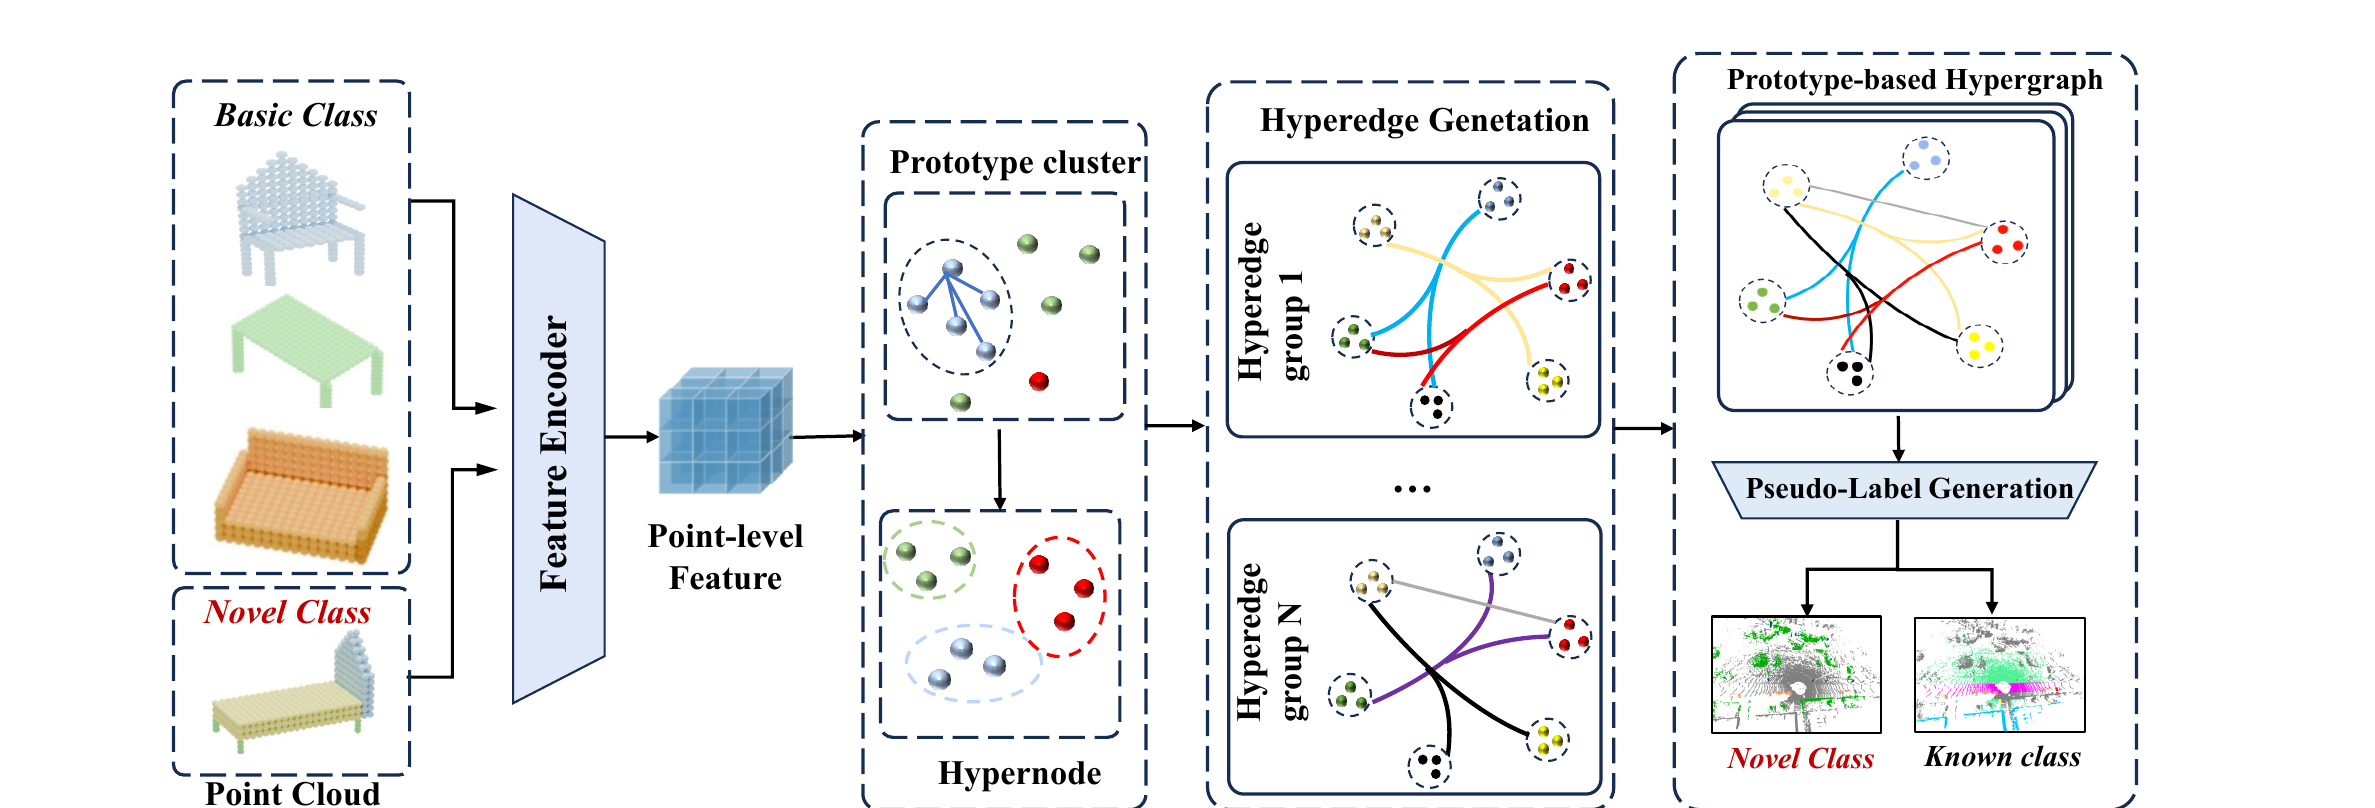
\includegraphics[width=0.75\linewidth]{imagenes/arq_hyperncd_paper.png}
\caption[Arquitectura de HyperNCD]{Arquitectura de HyperNCD. Fuente: Zhang et al.~\cite{zhang2026hyperncd},
Fig.~2.}
\label{fig:arq-hyperncd-paper}
\end{figure}

HyperNCD~\cite{zhang2026hyperncd} resuelve el NCD en cuatro etapas, que la
Figura~\ref{fig:arq-hyperncd-paper} presenta de izquierda a derecha:

\begin{enumerate}\setlength{\itemsep}{2pt}
\item \textbf{Codificador de características} (\emph{Feature Encoder}). La nube,
con puntos de clases conocidas y novedosas mezclados, entra a una red troncal que
asigna a cada punto un vector de características (\emph{point-level feature}).
En la implementación es la MinkowskiUNet-34C que produce $f_{\mathrm{sem}}$.
\item \textbf{Agrupamiento en prototipos} (\emph{Prototype cluster}). Una
convolución unidimensional seguida de \emph{softmax} reparte los puntos entre $K$
prototipos (Sección~\ref{sec:prototipo}); cada prototipo pasa a ser un nodo del
hipergrafo (\emph{hypernode}).
\item \textbf{Generación de hiperaristas} (\emph{Hyperedge generation}). Cada
prototipo se une a sus $M$ más afines según la afinidad $S_b$ de la
Ec.~\eqref{eq:afinidad}, que combina parecido geométrico y semántico. En cada
lote se forma un grupo de hiperaristas.
\item \textbf{Hipergrafo de prototipos y pseudo-etiquetas}
(\emph{Prototype-based hypergraph}). Las hiperaristas se reajustan a medida que
llegan lotes nuevos. Un prototipo cuya afinidad con uno conocido supera un umbral
recibe la etiqueta de esa clase; si no, se considera novedoso y recibe una
etiqueta nueva. Esas pseudo-etiquetas vuelven al entrenamiento.
\end{enumerate}

La figura corresponde a la formulación del artículo. La implementación publicada
que este trabajo ejecuta realiza las tres primeras etapas, pero no el reajuste
dinámico de la cuarta, y asigna las pseudo-etiquetas con Sinkhorn-Knopp en lugar
del umbral (Sección~\ref{sec:aporte}). Además, en la implementación los nodos del hipergrafo son
regiones y no prototipos (Sección~\ref{sec:hiperarista}); este trabajo adopta esa
formulación.

La función que optimiza el entrenamiento ejecutado suma un término por punto y
uno por región,
\begin{equation}
\nom{Lt}{\mathcal{L}}=\nom{Lp}{\mathcal{L}_{\mathrm{pt}}}+\nom{beta}{\beta}\,\nom{Lr}{\mathcal{L}_{\mathrm{reg}}},\qquad
\mathcal{L}_{\mathrm{pt}}=\sum_{v=1}^{2}\frac{1}{|\mathcal{P}_v|}\sum_{i\in\mathcal{P}_v}\mathrm{CE}\!\left(10\,z_i^{(v)},\;y_i^{(\bar v)}\right),
\label{eq:perdida}
\end{equation}
donde $v=1,2$ indexa las dos vistas aumentadas de la misma escena, $\bar v$ es
la otra vista, CE es la entropía cruzada y el objetivo $y_i^{(\bar v)}$ es
\emph{one-hot} para los puntos de clases conocidas y la pseudo-etiqueta de
Sinkhorn-Knopp (Ec.~\eqref{eq:sk-plan}) para los demás. $\mathcal{L}_{\mathrm{reg}}$
tiene la misma forma, pero sobre las regiones, con las puntuaciones de
$\hat{F}^{(r)}$ (Ec.~\eqref{eq:hiper-agr}) frente a los prototipos novedosos.
El peso $\beta$ es el argumento \texttt{--alpha} del programa de entrenamiento,
que vale 1 en las corridas registradas; no debe confundirse con el $\alpha$ de la
afinidad $S_b$, que vale 0{,}5.

\subsection{Arquitectura de Sonata}
\label{sec:arq-sonata-paper}

\begin{figure}[!htbp]
\centering
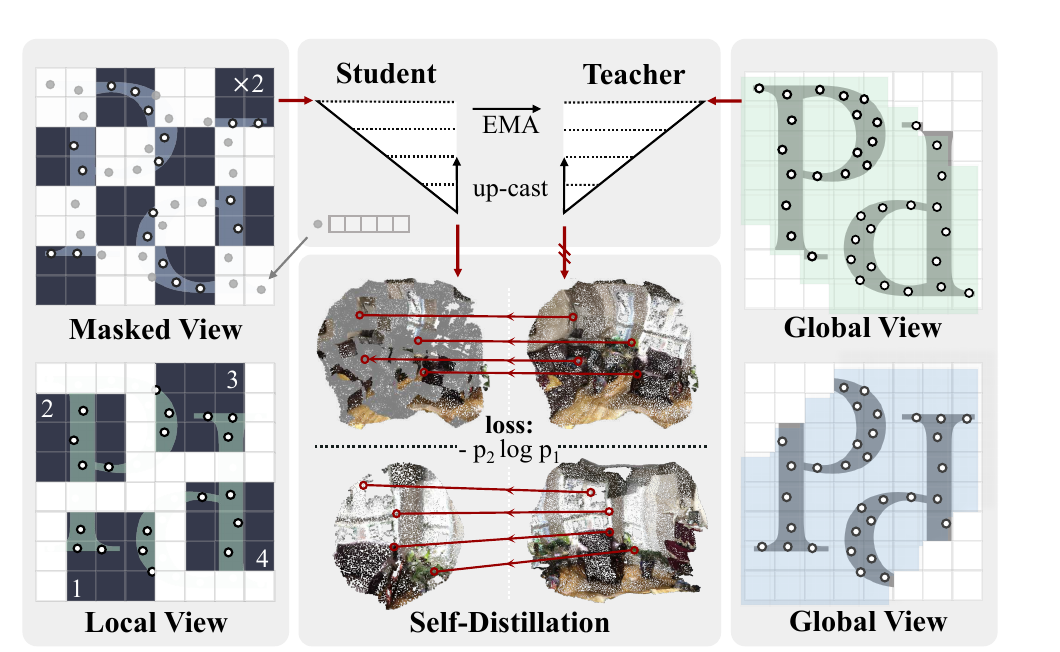
\includegraphics[width=0.62\linewidth]{imagenes/arq_sonata_paper.png}
\caption[Auto-destilación de Sonata]{Marco de auto-destilación de Sonata. Fuente: Wu et
al.~\cite{wu2025sonata}, Fig.~5.}
\label{fig:arq-sonata-paper}
\end{figure}

Sonata~\cite{wu2025sonata} no es un clasificador, sino un método para preentrenar
un codificador sin etiquetas. La Figura~\ref{fig:arq-sonata-paper} muestra cómo se
entrenó. Este trabajo no repite ese entrenamiento; usa únicamente el codificador
resultante, congelado. Del procedimiento interesan dos
propiedades, porque explican qué contiene $f_{\mathrm{ssl}}$:

\begin{itemize}\setlength{\itemsep}{2pt}
\item \textbf{Auto-destilación.} Dos copias de la misma red, estudiante y
maestro, reciben vistas distintas de una escena, y el estudiante aprende a
reproducir lo que el maestro dice de cada punto. Como el estudiante ve menos
contexto que el maestro, para acertar tiene que aprender qué es el punto y no
solo su geometría local.
\item \textbf{Codificador sin decodificador y \emph{up-cast}.} La red es un PTv3
al que se le quitó el decodificador, porque este favorecía el atajo geométrico
(Sección~\ref{sec:atajo}); para conservar información de varias escalas, las
características se devuelven a la resolución de las etapas anteriores mediante
el \emph{up-cast} (Sección~\ref{sec:upcast}).
\end{itemize}


% =====================================================================
\section{Métricas de Evaluación de Modelos}
\label{sec:metricas}

Para evaluar la efectividad del modelo se utilizan las métricas siguientes.


\subsection{IoU, mIoU y Clase Dominante}
\label{sec:iou}

Para una clase $c$, la intersección sobre unión se define como:
\begin{equation}
\nom{iou}{\mathrm{IoU}_c}=\frac{\nom{tp}{TP_c}}{\nom{tp}{TP_c}+\nom{tp}{FP_c}+\nom{tp}{FN_c}},
\label{eq:iou}
\end{equation}
Mide cuánto coinciden los puntos predichos de una clase con los reales: vale 1
si coinciden todos y 0 si no coincide ninguno.


\paragraph*{IoU Media (mIoU)}\phantomsection
\label{sec:miou}

La métrica agregada es el promedio de la anterior sobre un conjunto de clases:
\begin{equation}
\nom{miou}{\mathrm{mIoU}}(\nom{conj}{\mathcal{S}})=\frac{1}{\nom{card}{|}\nom{conj}{\mathcal{S}}\nom{card}{|}}\nomop{suma}{\sum}_{c\in\mathcal{S}}\nom{iou}{\mathrm{IoU}_c},
\qquad
\nom{conj}{\mathcal{S}}\nom{en}{\in}\{\nom{Ck}{\mathcal{C}_k},\;\nom{Cn}{\mathcal{C}_n},\;\nom{Ctodo}{\mathcal{C}}\}.
\label{eq:miou}
\end{equation}
Resume en un solo número el desempeño sobre todas las clases del conjunto.
Se reporta por separado como mIoU \emph{known}, mIoU \emph{novel} y mIoU
\emph{all}.

\paragraph*{Análisis de Dominancia}\phantomsection
\label{sec:dominancia}

La Ec.~\eqref{eq:miou} es una media aritmética no ponderada: cada clase pesa
igual con independencia de su número de puntos. Por ello el valor agregado se
acompaña siempre de la clase dominante:
\begin{equation}
\nom{cstar}{c^{*}}=\nomop{argmax}{\arg\max}_{c\in\mathcal{S}}\bigl|\nom{iou}{\mathrm{IoU}_c}-\nom{miou}{\mathrm{mIoU}}(\nom{conj}{\mathcal{S}})\bigr|.
\label{eq:dominante}
\end{equation}
Identifica la clase que más se aparta del promedio y que, por tanto, más
explica su valor.

\subsection{Medidas de Agrupamiento}
\label{sec:hungaro}

Como las clases de $\mathcal{C}_n$ se descubren sin etiqueta, la correspondencia
entre agrupaciones predichas y clases reales se resuelve por asignación óptima:
\begin{equation}
\nom{sigstar}{\sigma^{*}}=\nomop{argmax}{\arg\max}_{\sigma\in\mathfrak{S}_{|\mathcal{C}_n|}}
\nomop{suma}{\sum}_{c\in\mathcal{C}_n}\nom{iou}{\mathrm{IoU}}\bigl(\nom{y}{\hat{y}}=\nom{perm}{\sigma}(\nom{clase}{c}),\;\nom{ytrue}{y}=\nom{clase}{c}\bigr).
\label{eq:hungaro}
\end{equation}
Entre todas las correspondencias posibles elige la de mayor IoU total, y así
cada grupo descubierto recibe el nombre de una clase real.

\paragraph*{Índice de Rand Ajustado (ARI)}\phantomsection
\label{sec:ari}

Mide la coincidencia entre la agrupación descubierta y la real con independencia
del emparejamiento:
\begin{equation}
\nom{ariv}{\mathrm{ARI}}=
\frac{\nomop{suma}{\sum}_{ij}\binom{\nom{ari}{n_{ij}}}{2}
-\Bigl[\nomop{suma}{\sum}_i\binom{\nom{ari}{a_i}}{2}\nomop{suma}{\sum}_j\binom{\nom{ari}{b_j}}{2}\Bigr]\big/\binom{\nom{ntotal}{n}}{2}}
{\tfrac{1}{2}\Bigl[\nomop{suma}{\sum}_i\binom{\nom{ari}{a_i}}{2}+\nomop{suma}{\sum}_j\binom{\nom{ari}{b_j}}{2}\Bigr]
-\Bigl[\nomop{suma}{\sum}_i\binom{\nom{ari}{a_i}}{2}\nomop{suma}{\sum}_j\binom{\nom{ari}{b_j}}{2}\Bigr]\big/\binom{\nom{ntotal}{n}}{2}},
\label{eq:ari}
\end{equation}
Vale 1 cuando las dos agrupaciones coinciden y cerca de 0 cuando coinciden
solo por azar.


\paragraph*{Información Mutua Normalizada (NMI)}\phantomsection
\label{sec:nmi}

Complementa al ARI midiendo la información que una agrupación aporta sobre la
otra:
\begin{equation}
\nom{nmiv}{\mathrm{NMI}}(\nom{UV}{U},\nom{UV}{V})=\frac{2\,\nom{nmi}{I}(\nom{UV}{U};\nom{UV}{V})}{\nom{nmi}{H}(\nom{UV}{U})+\nom{nmi}{H}(\nom{UV}{V})},
\label{eq:nmi}
\end{equation}
Vale 1 cuando conocer una agrupación determina la otra y 0 cuando son
independientes.


\subsection{Linear Probing}
\label{sec:probing}

Protocolo de evaluación de un descriptor congelado, en el que se entrena únicamente un
clasificador lineal \nom{probe}{$W$} sobre él,
\begin{equation}
\nom{y}{\hat{y}_i}=\nomop{argmax}{\arg\max}\left(\nom{probe}{W}^{\nom{T}{\top}}\nom{fssl}{f_{\mathrm{ssl}}}(\nom{xi}{x^i})+\nom{probe}{b}\right),
\label{eq:probe}
\end{equation}
que asigna a cada punto la clase con mayor puntuación. Como el descriptor está
congelado, el desempeño resultante queda atribuido a la representación y no al
clasificador.

\subsection{Medidas de la Mejora}
\label{sec:ganancia}

Diferencia de mIoU sobre las clases novedosas entre el modelo híbrido y la línea
base:
\begin{equation}
\nom{delta}{\Delta\mathrm{mIoU}^{\mathrm{novel}}}=
\nom{supsub}{\mathrm{mIoU}^{\mathrm{novel}}_{\mathrm{hib}}}-\nom{supsub}{\mathrm{mIoU}^{\mathrm{novel}}_{\mathrm{base}}}.
\label{eq:delta}
\end{equation}
Indica cuántos puntos de mIoU gana, o pierde, el modelo híbrido en las clases
novedosas.

\paragraph*{Brecha Cerrada}\phantomsection
\label{sec:brecha}

La ganancia absoluta no es interpretable por sí sola, porque el techo alcanzable
depende de la sección. Esta métrica, propuesta en el presente trabajo, la
normaliza por la brecha que separa a la línea base de su propio desempeño sobre
las clases que sí vio etiquetadas:
\begin{equation}
\nom{G}{G}=\frac{\nom{supsub}{\mathrm{mIoU}^{\mathrm{novel}}_{\mathrm{hib}}}-\nom{supsub}{\mathrm{mIoU}^{\mathrm{novel}}_{\mathrm{base}}}}
{\nom{supsub}{\mathrm{mIoU}^{\mathrm{known}}_{\mathrm{base}}}-\nom{supsub}{\mathrm{mIoU}^{\mathrm{novel}}_{\mathrm{base}}}}.
\label{eq:G}
\end{equation}
\nom{G}{$G$} es adimensional. $G=0$ indica que la sustitución no aporta, $G=1$ que las
clases novedosas alcanzan la calidad con que el modelo segmenta las conocidas y
$G<0$ degradación.

\paragraph*{Atribución por Etapas}\phantomsection
\label{sec:metricas-hibrido}

Como el proceso es separable en dos etapas, la métrica se reporta también en el
punto intermedio y no solo al final, con \emph{linear probing} sobre el descriptor
(Ec.~\eqref{eq:probe}) antes de la formación de prototipos y mIoU
(Ec.~\eqref{eq:miou}) después. Esa separación permite atribuir una mejora a la
representación o al razonamiento, y no al sistema tratado como caja negra.

% =====================================================================
\section{Diseño de la Tesis}
\label{sec:diseno-teorico}

La Figura~\ref{fig:diseno} organiza el sistema en cinco módulos; sobre cada
flecha se indica lo que pasa de un módulo al siguiente. El diagrama muestra solo
imágenes y fórmulas. Cada fórmula enlaza con su ecuación en el marco teórico,
donde se explica, y allí cada símbolo enlaza con su fila en la nomenclatura del
\hyperref[sec:anexo-nomenclatura]{Anexo~B}. El diagrama representa el
diseño del sistema; todas las conexiones mostradas están implementadas y se
ejecutaron sobre datos reales (Sección~\ref{sec:estado-impl}).

\begin{figure}[!t]
\centering
{\hypersetup{linkcolor=blue!55!black}\fuentediagrama
\makebox[\linewidth][c]{\adjustbox{max width=1.12\linewidth, max totalheight=0.85\textheight}{% Diagrama de diseno: cinco modulos; el Modulo 4 contiene sus cuatro operaciones.
% Solo imagenes y formulas; cada formula enlaza con su ecuacion en el marco teorico.
% Modulo 1 segun preprocesar.py; entradas de los Modulos 2 y 3 segun el codigo.
% Flecha continua: conexion implementada. Todas las conexiones estan implementadas.
% Cada linea y cada formula enlaza con el marco teorico (correspondencia uno a uno).
% La incluyen la tesis (capitulo2.tex) y diagrama_diseno.tex (PDF/PNG).
\definecolor{cEnt}{RGB}{31,78,121}
\definecolor{cSem}{RGB}{31,110,60}
\definecolor{cEnc}{RGB}{101,60,140}
\definecolor{cFus}{RGB}{176,32,42}
\definecolor{cSal}{RGB}{191,110,20}
\pgfdeclarelayer{background}
\pgfsetlayers{background,main}
\begin{tikzpicture}[
  font=\scriptsize,
  execute at begin node={\hyphenpenalty=10000\exhyphenpenalty=10000},
  mod/.style={rounded corners=3pt, draw, thick, align=center, inner sep=5pt},
  tab/.style={rounded corners=2pt, text=white, font=\scriptsize\bfseries, inner sep=3pt, anchor=south, align=center},
  tarj/.style={rounded corners=2.5pt, draw=black!40, fill=white, semithick,
               align=left, inner sep=4pt, text width=4.45cm, anchor=north},
  chico/.style={font=\tiny, text=black!65},
  fl/.style={-{Latex[length=2.1mm]}, thick, black!65},
  flp/.style={fl, densely dashed}
]
%% ---------- preprocesamiento ----------
\node[mod, draw=cEnt, fill=cEnt!6, text width=4.3cm, anchor=center] (M1) at (0,0)
 {{\rule{0pt}{8pt}\scriptsize\bfseries\itshape \hyperref[sec:tls]{\textcolor{cEnt}{levantamiento TLS}}}\\[4pt]
  \tikz[baseline=0, every node/.style={anchor=center, align=center, text width={}, minimum height=0pt, minimum width=0pt, inner sep=1pt}]{
    \draw[black!35] (0.34,0.23) rectangle (1.59,1.28);
    \draw[black!35] (0,0) -- (0.34,0.23) (1.25,0) -- (1.59,0.23) (1.25,1.05) -- (1.59,1.28) (0,1.05) -- (0.34,1.28);
    \foreach \x/\y/\t in {0.097/0.087/95, 0.089/0.121/98, 0.080/0.175/97, 0.104/0.235/93, 0.139/0.278/89, 0.129/0.332/87, 0.129/0.372/89, 0.106/0.408/92, 0.135/0.448/87, 0.142/0.512/86, 0.117/0.540/93, 0.159/0.598/85, 0.104/0.595/97, 0.101/0.671/94, 0.121/0.703/92, 0.118/0.750/91, 0.132/0.815/89, 0.168/0.875/84, 0.148/0.892/86, 0.139/0.944/90, 0.148/0.980/87, 0.087/0.988/98, 0.163/0.103/93, 0.165/0.134/93, 0.198/0.218/83, 0.129/0.216/96, 0.215/0.297/82, 0.233/0.353/79, 0.179/0.362/87, 0.155/0.397/91, 0.150/0.427/95, 0.226/0.521/80, 0.191/0.543/88, 0.187/0.597/87, 0.213/0.657/81, 0.195/0.685/85, 0.204/0.736/81, 0.145/0.742/95, 0.141/0.786/95, 0.152/0.835/94, 0.197/0.904/85, 0.191/0.955/85, 0.174/0.976/87, 0.193/1.022/88, 0.235/0.109/86, 0.242/0.163/83, 0.254/0.215/81, 0.241/0.260/82, 0.257/0.300/80, 0.227/0.325/86, 0.236/0.364/86, 0.231/0.430/85, 0.243/0.456/86, 0.244/0.522/85, 0.234/0.547/84, 0.255/0.623/80, 0.252/0.651/80, 0.236/0.690/86, 0.249/0.738/81, 0.227/0.767/86, 0.269/0.837/78, 0.261/0.870/78, 0.251/0.920/84, 0.239/0.953/87, 0.263/1.014/81, 0.231/1.026/86, 0.300/0.122/80, 0.263/0.160/88, 0.349/0.247/73, 0.323/0.279/78, 0.262/0.294/86, 0.298/0.354/81, 0.308/0.410/79, 0.324/0.447/75, 0.292/0.482/83, 0.315/0.539/76, 0.322/0.595/75, 0.279/0.600/87, 0.276/0.645/87, 0.297/0.694/81, 0.320/0.756/76, 0.258/0.755/87, 0.324/0.841/74, 0.317/0.867/80, 0.286/0.906/83, 0.299/0.960/82, 0.265/0.982/87, 0.297/1.051/82, 0.340/0.125/80, 0.359/0.188/79, 0.369/0.231/78, 0.374/0.282/74, 0.358/0.320/78, 0.369/0.370/75, 0.343/0.396/79, 0.368/0.456/78, 0.361/0.491/80, 0.385/0.541/72, 0.390/0.605/72, 0.374/0.634/76, 0.314/0.644/85, 0.318/0.694/85, 0.376/0.760/72, 0.377/0.801/73, 0.363/0.858/75, 0.381/0.904/75, 0.394/0.933/72, 0.336/0.961/83, 0.341/1.010/83, 0.381/1.078/72, 0.395/0.130/78, 0.418/0.197/75, 0.407/0.228/77, 0.419/0.271/74, 0.456/0.339/70, 0.429/0.386/71, 0.427/0.415/74, 0.402/0.452/79, 0.438/0.526/69, 0.438/0.555/71, 0.390/0.567/79, 0.406/0.616/78, 0.414/0.680/77, 0.455/0.737/68, 0.405/0.745/78, 0.397/0.800/77, 0.398/0.838/77, 0.467/0.912/66, 0.419/0.941/75, 0.438/0.997/73, 0.447/1.050/69, 0.452/1.099/67, 0.458/0.140/76, 0.518/0.231/64, 0.468/0.227/76, 0.485/0.291/69, 0.472/0.335/75, 0.485/0.372/72, 0.457/0.393/77, 0.479/0.455/73, 0.445/0.491/79, 0.472/0.551/72, 0.501/0.620/65, 0.447/0.624/77, 0.443/0.670/78, 0.462/0.722/77, 0.512/0.785/67, 0.499/0.821/69, 0.467/0.858/75, 0.499/0.926/69, 0.479/0.938/72, 0.486/1.006/69, 0.491/1.035/69, 0.511/1.090/65, 0.568/0.177/63, 0.537/0.215/67, 0.546/0.262/67, 0.507/0.277/74, 0.537/0.358/66, 0.523/0.385/72, 0.551/0.443/64, 0.499/0.459/74, 0.528/0.506/72, 0.549/0.574/66, 0.499/0.594/75, 0.497/0.618/76, 0.518/0.683/74, 0.540/0.744/66, 0.549/0.791/68, 0.499/0.805/74, 0.511/0.855/74, 0.490/0.895/77, 0.574/0.987/62, 0.534/1.003/68, 0.550/1.064/67, 0.525/1.094/70, 0.550/0.153/75, 0.590/0.219/68, 0.562/0.243/73, 0.584/0.290/68, 0.592/0.348/67, 0.570/0.383/73, 0.559/0.416/75, 0.548/0.450/74, 0.571/0.524/71, 0.568/0.553/73, 0.624/0.633/61, 0.578/0.652/70, 0.618/0.726/62, 0.580/0.746/68, 0.541/0.751/75, 0.574/0.818/68, 0.583/0.869/69, 0.585/0.909/68, 0.568/0.942/73, 0.585/1.003/70, 0.586/1.052/67, 0.554/1.063/73, 0.607/0.721/73, 0.602/0.781/71, 0.670/0.851/61, 0.609/0.856/71, 0.629/0.914/69, 0.653/0.989/60, 0.600/0.970/74, 0.586/1.018/74, 0.647/1.116/61, 0.652/0.765/72, 0.697/0.844/64, 0.648/0.858/72, 0.679/0.905/68, 0.654/0.948/73, 0.679/1.022/65, 0.682/1.057/68, 0.674/1.092/70, 0.757/0.840/62, 0.688/0.860/71, 0.736/0.927/65, 0.692/0.985/73, 0.749/1.066/63, 0.708/1.092/68, 0.799/0.847/61, 0.797/0.884/62, 0.766/0.915/65, 0.719/0.937/75, 0.751/0.988/71, 0.747/1.041/72, 0.741/1.081/70, 0.813/0.847/66, 0.780/0.836/75, 0.783/0.986/71, 0.783/1.026/71, 0.825/1.108/64, 0.822/0.776/73, 0.822/0.794/76, 0.852/0.872/67, 0.840/0.917/71, 0.816/0.949/72, 0.851/1.015/66, 0.809/1.033/74, 0.860/1.109/66, 0.848/0.757/75, 0.820/0.786/81, 0.827/0.845/80, 0.900/0.906/68, 0.834/0.922/81, 0.826/0.974/79, 0.878/1.052/69, 0.851/1.084/74, 0.881/0.706/79, 0.865/0.745/83, 0.913/0.823/73, 0.905/0.869/73, 0.859/0.864/82, 0.872/0.938/79, 0.857/0.934/86, 0.927/1.043/72, 0.908/1.070/75, 0.902/0.128/82, 0.895/0.167/84, 0.900/0.202/85, 0.945/0.285/74, 0.944/0.325/78, 0.893/0.349/85, 0.924/0.403/77, 0.895/0.428/85, 0.919/0.472/83, 0.949/0.554/75, 0.922/0.569/80, 0.931/0.626/76, 0.943/0.656/77, 0.902/0.703/84, 0.936/0.762/75, 0.927/0.804/78, 0.911/0.824/81, 0.922/0.876/79, 0.894/0.898/88, 0.917/0.963/79, 0.894/0.986/84, 0.912/1.038/81, 0.963/0.124/83, 0.974/0.185/80, 0.911/0.189/91, 0.943/0.239/87, 0.923/0.267/91, 0.914/0.314/93, 0.896/0.353/92, 0.928/0.400/90, 0.932/0.463/86, 0.936/0.509/87, 0.947/0.578/82, 0.951/0.610/81, 0.911/0.602/94, 0.967/0.701/80, 0.938/0.717/88, 0.919/0.767/90, 0.948/0.812/83, 0.933/0.876/84, 0.921/0.879/90, 0.941/0.959/85, 0.947/1.013/83, 0.925/1.017/89, 0.972/0.091/90, 0.985/0.154/86, 0.987/0.207/87, 0.955/0.221/90, 0.988/0.289/83, 0.991/0.353/82, 0.951/0.374/90, 0.927/0.381/96, 0.989/0.466/84, 0.962/0.477/92, 0.945/0.521/93, 0.949/0.583/91, 0.954/0.621/89, 0.980/0.674/87, 0.968/0.727/87, 0.952/0.763/90, 0.974/0.811/88, 0.984/0.849/85, 0.975/0.891/89, 0.974/0.956/86, 0.995/1.012/82, 0.961/1.036/89, 0.973/0.090/95, 0.964/0.115/100, 0.988/0.185/94, 0.986/0.227/94, 1.012/0.282/89, 1.003/0.313/89, 1.018/0.365/88, 1.030/0.418/87, 0.979/0.434/97, 0.999/0.503/89, 0.992/0.531/92, 0.990/0.581/92, 0.991/0.608/92, 0.963/0.650/98, 0.981/0.691/95, 0.958/0.714/100, 0.989/0.783/93, 0.987/0.828/92, 0.996/0.885/94, 0.971/0.900/97, 0.959/0.960/99, 0.991/1.002/96, 0.988/0.076/100, 0.993/0.106/100, 1.031/0.193/92, 0.989/0.198/100, 0.997/0.244/100, 1.001/0.300/100, 1.030/0.337/96, 1.001/0.379/99, 1.020/0.431/98, 1.039/0.482/93, 1.016/0.522/96, 0.989/0.532/100, 1.035/0.606/94, 1.039/0.675/92, 0.985/0.663/100, 1.045/0.760/91, 1.044/0.794/90, 1.035/0.831/94, 1.021/0.877/94, 0.989/0.882/100, 0.990/0.945/100, 1.027/1.003/92, 1.074/0.088/94, 1.056/0.111/98, 1.046/0.159/97, 1.036/0.187/100, 1.008/0.234/100, 1.066/0.293/97, 1.026/0.324/100, 1.057/0.386/96, 1.031/0.405/100, 1.039/0.460/99, 1.025/0.495/100, 1.021/0.530/100, 1.018/0.583/100, 1.055/0.643/99, 1.038/0.673/100, 1.058/0.726/96, 1.070/0.775/95, 1.037/0.809/100, 1.010/0.853/100, 1.010/0.893/100, 1.021/0.928/100, 1.011/0.956/100, 1.081/0.050/100, 1.040/0.083/100, 1.067/0.133/100, 1.037/0.163/100, 1.102/0.239/98, 1.037/0.272/100, 1.062/0.327/100, 1.080/0.364/100, 1.061/0.411/100, 1.043/0.411/100, 1.064/0.497/100, 1.062/0.530/100, 1.032/0.559/100, 1.046/0.618/100, 1.056/0.653/100, 1.102/0.737/98, 1.054/0.738/100, 1.065/0.798/100, 1.045/0.819/100, 1.060/0.880/100, 1.067/0.944/100, 1.031/0.950/100, 1.089/0.041/100, 1.079/0.066/100, 1.098/0.129/100, 1.069/0.160/100, 1.091/0.210/100, 1.073/0.245/100, 1.108/0.320/100, 1.130/0.358/100, 1.135/0.420/100, 1.117/0.465/100, 1.120/0.507/100, 1.120/0.555/100, 1.073/0.546/100, 1.087/0.599/100, 1.076/0.656/100, 1.073/0.706/100, 1.077/0.746/100, 1.069/0.788/100, 1.070/0.831/100, 1.088/0.859/100, 1.094/0.924/100, 1.079/0.954/100, 1.150/0.055/100, 1.113/0.052/100, 1.153/0.136/100, 1.137/0.177/100, 1.086/0.187/100, 1.118/0.234/100, 1.164/0.307/100, 1.093/0.327/100, 1.122/0.372/100, 1.110/0.417/100, 1.084/0.453/100, 1.108/0.494/100, 1.109/0.541/100, 1.114/0.592/100, 1.141/0.661/100, 1.123/0.697/100, 1.143/0.744/100, 1.126/0.776/100, 1.122/0.810/100, 1.126/0.856/100, 1.121/0.907/100, 1.102/0.944/100} \fill[cEnt!\t] (\x,\y) circle (0.013);
    \draw[black!55, semithick] (0,0) rectangle (1.25,1.05);}\\[5pt]
  \begin{minipage}{\linewidth}\centering\scriptsize
  \adjustbox{max width=\linewidth}{\enlaceec{eq:centrado}{$x_i'=x_i-c$}}\\[4pt]
  \adjustbox{max width=\linewidth}{\enlaceec{eq:sor}{$\bar d_i\le\mu+\lambda\,\sigma$}}\\[4pt]
  \adjustbox{max width=\linewidth}{\enlaceec{eq:voxel}{$\bar x_v=\frac{1}{|v|}\sum_{i\in v}x_i$}}\\[4pt]
  \adjustbox{max width=\linewidth}{\enlaceec{eq:normal}{$C=\frac{1}{q}\sum_{j}(p_j-\bar p)(p_j-\bar p)^{\top}$}}\\[4pt]
  \adjustbox{max width=\linewidth}{\enlaceec{eq:sj}{$S=[\,x,y,z,R,G,B,n_x,n_y,n_z\,]$}}
\end{minipage}};

%% ---------- semantica y encoder ----------
\node[mod, draw=cSem, fill=cSem!6, text width=5.0cm, anchor=south] (M2) at ($(M1.north)+(1.6,1.6)$)
 {{\rule{0pt}{8pt}\scriptsize\bfseries\itshape \hyperref[sec:arq-hyperncd-paper]{\textcolor{cSem}{HyperNCD}}}\\[4pt]
  \tikz[baseline=0, every node/.style={anchor=center, align=center, text width={}, minimum height=0pt, minimum width=0pt, inner sep=1pt}]{
    \foreach \i/\h in {0/0.95, 1/0.72, 2/0.50, 3/0.32}
      \fill[cSem!35, draw=cSem] (\i*0.24,0.5-\h/2) rectangle (\i*0.24+0.16,0.5+\h/2);
    \foreach \i/\h in {0/0.32, 1/0.50, 2/0.72, 3/0.95}
      \fill[cSem!65, draw=cSem] (1.1+\i*0.24,0.5-\h/2) rectangle (1.1+\i*0.24+0.16,0.5+\h/2);
    \foreach \a/\b/\h in {0/3/0.95, 1/2/0.72, 2/1/0.50}
      \draw[cSem!80, densely dashed, -{Latex[length=1mm]}] (\a*0.24+0.16,0.5+\h/2+0.05) -- (1.1+\b*0.24,0.5+\h/2+0.05);
    \draw[-{Latex[length=1.2mm]}, cSem!80, semithick] (0.88,0.5) -- (1.08,0.5);}\\[5pt]
  \begin{minipage}{\linewidth}\centering\scriptsize
  \adjustbox{max width=\linewidth}{\enlaceec{eq:cuant}{$\mathbf{v}_i=\lfloor x_i/\ell\rfloor,\; a_{\mathbf{v}}=1$}}\\[4pt]
  \adjustbox{max width=\linewidth}{\enlaceec{eq:fsem}{$f_{\mathrm{sem}}(x^i)=U_\theta(\mathcal{V})_{\mathbf{v}_i}\in\mathbb{R}^{96}$}}\\[4pt]
  \adjustbox{max width=\linewidth}{\enlaceec{eq:cabeza}{$z_{i,k}=\frac{\langle f_{\mathrm{sem}}(x^i),w_k\rangle}{\lVert f_{\mathrm{sem}}(x^i)\rVert\,\lVert w_k\rVert}$}}\\[4pt]
  \adjustbox{max width=\linewidth}{\enlaceec{eq:sk-plan}{$Y=B\,\mathrm{diag}(u)\,Q\,\mathrm{diag}(v)$}}\\[4pt]
  \adjustbox{max width=\linewidth}{\enlaceec{eq:g-region}{$g^{(r)}=\left[\frac{\lambda_1-\lambda_2}{\lambda_1},\frac{\lambda_2-\lambda_3}{\lambda_1},\frac{\lambda_3}{\lambda_1},c^{(r)}\right]$}}\\[4pt]
  \adjustbox{max width=\linewidth}{\enlaceec{eq:hiper-agr}{$\hat F^{(r)}=\sum_{j\in\mathcal{N}_M(r)}\tilde S_{rj}F^{(j)}$}}\\[4pt]
  \adjustbox{max width=\linewidth}{\enlaceec{eq:perdida}{$\mathcal{L}=\mathcal{L}_{\mathrm{pt}}+\beta\,\mathcal{L}_{\mathrm{reg}}$}}
\end{minipage}};

\node[mod, draw=cEnc, fill=cEnc!6, text width=6.4cm, anchor=north] (M3) at ($(M1.south)+(0.2,-1.75)$)
 {{\rule{0pt}{8pt}\scriptsize\bfseries\itshape \hyperref[sec:arq-sonata-paper]{\textcolor{cEnc}{Sonata}}}\\[4pt]
  \tikz[baseline=0, every node/.style={anchor=center, align=center, text width={}, minimum height=0pt, minimum width=0pt, inner sep=1pt}]{
    \foreach \i/\w in {0/1.15, 1/0.97, 2/0.79, 3/0.61, 4/0.43}
      \fill[rounded corners=1pt, cEnc!45, draw=cEnc] (0,\i*0.19) rectangle (\w,\i*0.19+0.13);
    \begin{scope}[shift={(1.55,0.5)}]
      \foreach \a in {0,60,120}{
        \draw[cyan!65!black, thick] ({\a}:-0.26) -- ({\a}:0.26);
        \foreach \s in {1,-1}{ \draw[cyan!65!black, semithick] ({\a}:0.17*\s) -- ++({\a+40*\s}:0.08); \draw[cyan!65!black, semithick] ({\a}:0.17*\s) -- ++({\a-40*\s}:0.08);}}
    \end{scope}}\\[5pt]
  \begin{minipage}{\linewidth}\centering\scriptsize
  \adjustbox{max width=\linewidth}{\enlaceec{eq:embedding}{$\mathbf{h}_i^{(0)}=\mathrm{GELU}(\mathrm{LN}(W_e\mathbf{x}_i+b_e))$}}\\[4pt]
  \adjustbox{max width=\linewidth}{\enlaceec{eq:atencion}{$\mathrm{Atn}(\mathbf{H}_p)=\mathrm{softmax}\big(\mathbf{H}_pW_Q(\mathbf{H}_pW_K)^{\top}\!/\sqrt{d}\big)\,\mathbf{H}_pW_V$}}\\[4pt]
  \adjustbox{max width=\linewidth}{\enlaceec{eq:upcast}{$f_{\mathrm{ssl}}(x^i)=[\mathbf{h}^{(3)};\mathbf{h}^{(4)};\mathbf{h}^{(5)}]_{\mathrm{inv}(i)}\in\mathbb{R}^{1088}$}}\\[4pt]
  \adjustbox{max width=\linewidth}{\enlaceec{eq:probe}{$\hat{y}_i=\arg\max\left(W^{\top}f_{\mathrm{ssl}}(x^i)+b\right)$}}
\end{minipage}};

%% ---------- fusion ----------
\node[align=center, anchor=north, text width=4.8cm] (M4h) at (8.35,9.2)
 {{\rule{0pt}{8pt}\scriptsize\bfseries\itshape \hyperref[sec:arq-hyperncd-paper]{\textcolor{cFus}{HyperNCD}}}};

\node[tarj] (T1) at ($(M4h.south)+(0,-0.3)$)
 {\enlace{sec:concat}{\textbf{\textcircled{\scriptsize 1} Concatenación}}\\[3pt]
  \begin{minipage}{\linewidth}\centering
  \adjustbox{max width=\linewidth}{\tikz[baseline=0, every node/.style={anchor=center, align=center, text width={}, minimum height=0pt, minimum width=0pt, inner sep=1pt}]{
    \fill[cSem!45, draw=cSem] (0,0) rectangle (0.36,0.22);
    \fill[cEnc!45, draw=cEnc] (0.36,0) rectangle (2.2,0.22);
    \node[font=\tiny] at (0.18,0.11) {\hyperref[sec:fsem]{96}};
    \node[font=\tiny] at (1.28,0.11) {\hyperref[sec:fssl]{1088}};
    \fill[cSem!45, draw=cSem] (2.45,0) rectangle (2.81,0.22);
    \fill[red!30, draw=cFus] (2.81,0) rectangle (2.93,0.22);
    \node[font=\tiny, text=black!60] at (2.69,-0.16) {\hyperref[sec:fgeo]{antes}};}}\\[4pt]
  \enlaceec{eq:hibrido}{$F_i=\left[\,f_{\mathrm{sem}};\,f_{\mathrm{ssl}}\,\right]$}\\[4pt]
  \adjustbox{max width=\linewidth}{\enlaceec{eq:reg-prom}{$F^{(r)}=\frac{1}{|r|}\sum_{i\in r}F_i$}}\end{minipage}};

\node[tarj] (T2) at ($(T1.south)+(0,-1.0)$)
 {\enlace{sec:afinhiper}{\textbf{\textcircled{\scriptsize 2} Afinidad entre regiones}}\\[3pt]
  \begin{minipage}{\linewidth}\centering
  \adjustbox{max width=\linewidth}{\tikz[baseline=0, every node/.style={anchor=center, align=center, text width={}, minimum height=0pt, minimum width=0pt, inner sep=1pt}]{\begin{scope}[scale=0.85]
    \fill[cSem!25, draw=cSem!60, rotate=20] (0.72,0.26) ellipse (0.80 and 0.34);
    \fill[cEnc!25, draw=cEnc!60, rotate=-15] (1.42,0.52) ellipse (0.74 and 0.32);
    \foreach \x/\y in {0.25/0.20, 0.72/0.46, 1.05/0.14, 1.55/0.40, 1.98/0.12, 1.62/0.70}
      \fill[black!75] (\x,\y) circle (0.05);\end{scope}}}\\[4pt]
  \adjustbox{max width=\linewidth}{\enlaceec{eq:coseno}{$S_s=\frac{\langle F^{(i)},F^{(j)}\rangle}{\lVert F^{(i)}\rVert\,\lVert F^{(j)}\rVert}$}}\\[4pt]
  \adjustbox{max width=\linewidth}{\enlaceec{eq:gauss}{$S_g=\exp\left(-\lVert g^{(i)}-g^{(j)}\rVert^{2}/\tau\right)$}}\\[4pt]
  \enlaceec{eq:afinidad}{$S_b=\alpha S_g+(1-\alpha)S_s$}\end{minipage}};

\node[tarj] (T3) at ($(T2.south)+(0,-1.0)$)
 {\enlace{sec:hiperarista}{\textbf{\textcircled{\scriptsize 3} Hiperaristas}}\\[3pt]
  \begin{minipage}{\linewidth}\centering
  \adjustbox{max width=\linewidth}{\enlaceec{eq:hiper-agr}{$\hat F^{(r)}=\sum_{j\in\mathcal{N}_M(r)}\tilde S_{rj}F^{(j)}$}}\end{minipage}};

\node[tarj] (T4) at ($(T3.south)+(0,-1.0)$)
 {\enlace{sec:formproto}{\textbf{\textcircled{\scriptsize 4} Prototipos y pseudo-etiquetas}}~\logo{pytorch.png}\\[3pt]
  \begin{minipage}{\linewidth}\centering
  \adjustbox{max width=\linewidth}{\tikz[baseline=0, every node/.style={anchor=center, align=center, text width={}, minimum height=0pt, minimum width=0pt, inner sep=1pt}]{\begin{scope}[scale=0.85]
    \foreach \x/\y/\c in {0.222/0.339/cSem, 0.457/0.245/cSem, 0.212/0.293/cSem, 0.401/0.416/cSem, 0.234/0.177/cSem, 0.429/0.353/cSem, 0.494/0.392/cSem, 0.330/0.247/cSem, 1.343/0.558/cEnc, 1.069/0.463/cEnc, 1.179/0.624/cEnc, 1.092/0.570/cEnc, 1.182/0.660/cEnc, 1.267/0.602/cEnc, 0.986/0.644/cEnc, 1.005/0.562/cEnc, 1.651/0.120/cSal, 1.712/0.144/cSal, 1.999/0.117/cSal, 1.884/-0.012/cSal, 1.766/0.197/cSal, 1.785/0.179/cSal, 1.811/0.011/cSal, 1.862/0.031/cSal} \fill[\c!55] (\x,\y) circle (0.035);
    \foreach \x/\y/\c in {0.35/0.30/cSem, 1.15/0.58/cEnc, 1.80/0.12/cSal}
      \node[star, star points=5, star point ratio=2.2, draw=\c, fill=\c!35, inner sep=0.6pt] at (\x,\y) {};\end{scope}}}\\[4pt]
  \adjustbox{max width=\linewidth}{\enlaceec{eq:prototipo}{$P_k=\frac{\sum_{i}s_{i,k}F_i}{\sum_{i}s_{i,k}}$}}\\[4pt]
  \adjustbox{max width=\linewidth}{\enlaceec{eq:sk-costo}{$Q_{ik}=\mathrm{softmax}(o_i/0{,}1)_k^{1/\epsilon_{\mathrm{sk}}}$}}\\[4pt]
  \adjustbox{max width=\linewidth}{\enlaceec{eq:sk-iter}{$u\leftarrow\frac{1/B}{Qv},\;v\leftarrow\left(\frac{1/|\mathcal{C}_n|}{Q^{\top}u}\right)^{\frac{\gamma}{\gamma+\epsilon_{\mathrm{sk}}}}$}}\\[4pt]
  \adjustbox{max width=\linewidth}{\enlaceec{eq:sk-plan}{$Y=B\,\mathrm{diag}(u)\,Q\,\mathrm{diag}(v)$}}\end{minipage}};

\begin{pgfonlayer}{background}
\node[fit=(M4h)(T1)(T2)(T3)(T4), draw=cFus, very thick, fill=cFus!5,
      rounded corners=3pt, inner sep=7pt] (M4) {};
\end{pgfonlayer}
\draw[fl] (T1.south) -- (T2.north)
  node[midway, right=0.6mm, chico, align=left, fill=cFus!5, inner sep=1pt]
  {\hyperref[sec:region]{regiones de}\\\hyperref[sec:region]{0{,}75\,m}};
\draw[fl] (T2.south) -- (T3.north)
  node[midway, right=0.6mm, chico, align=left, fill=cFus!5, inner sep=1pt]
  {\hyperref[eq:afinidad]{$S_b$ entre}\\\hyperref[sec:hipergrafo]{regiones}};
\draw[fl] (T3.south) -- (T4.north)
  node[midway, right=0.6mm, chico, align=left, fill=cFus!5, inner sep=1pt]
  {\hyperref[sec:hipergrafo]{hipergrafo $\mathcal{H}$}\\\hyperref[eq:hiper-agr]{$\hat F^{(r)}$}};

%% ---------- salida ----------
\node[mod, draw=cSal, fill=cSal!6, text width=4.35cm, anchor=west] (M5) at ($(M4.east)+(1.3,0)$)
 {{\rule{0pt}{8pt}\scriptsize\bfseries\itshape \hyperref[sec:modulo5]{\textcolor{cSal}{evaluación y plataforma}}}\\[4pt]
  \tikz[baseline=0, every node/.style={anchor=center, align=center, text width={}, minimum height=0pt, minimum width=0pt, inner sep=1pt}]{
    \draw[black!35] (0.34,0.23) rectangle (1.59,1.28);
    \draw[black!35] (0,0) -- (0.34,0.23) (1.25,0) -- (1.59,0.23) (1.25,1.05) -- (1.59,1.28) (0,1.05) -- (0.34,1.28);
    \foreach \x/\y/\c in {0.097/0.087/cSal, 0.089/0.121/cSal, 0.080/0.175/cSem, 0.104/0.235/cSem, 0.139/0.278/cSem, 0.129/0.332/cSem, 0.129/0.372/cSem, 0.106/0.408/cSem, 0.135/0.448/cSem, 0.142/0.512/cSem, 0.117/0.540/cSem, 0.159/0.598/cSem, 0.104/0.595/cSem, 0.101/0.671/cSem, 0.121/0.703/cSem, 0.118/0.750/cSem, 0.132/0.815/cSem, 0.168/0.875/cSem, 0.148/0.892/cSem, 0.139/0.944/cSem, 0.148/0.980/cSem, 0.087/0.988/cSem, 0.163/0.103/cSal, 0.165/0.134/cSal, 0.198/0.218/cSem, 0.129/0.216/cSem, 0.215/0.297/cSem, 0.233/0.353/cSem, 0.179/0.362/cSem, 0.155/0.397/cSem, 0.150/0.427/cSem, 0.226/0.521/cSem, 0.191/0.543/cSem, 0.187/0.597/cSem, 0.213/0.657/cSem, 0.195/0.685/cSem, 0.204/0.736/cSem, 0.145/0.742/cSem, 0.141/0.786/cSem, 0.152/0.835/cSem, 0.197/0.904/cSem, 0.191/0.955/cSem, 0.174/0.976/cSem, 0.193/1.022/cSem, 0.235/0.109/cSal, 0.242/0.163/cSal, 0.254/0.215/cSem, 0.241/0.260/cSem, 0.257/0.300/cSem, 0.227/0.325/cSem, 0.236/0.364/cSem, 0.231/0.430/cSem, 0.243/0.456/cSem, 0.244/0.522/cSem, 0.234/0.547/cSem, 0.255/0.623/cSem, 0.252/0.651/cSem, 0.236/0.690/cSem, 0.249/0.738/cSem, 0.227/0.767/cSem, 0.269/0.837/cSem, 0.261/0.870/cSem, 0.251/0.920/cSem, 0.239/0.953/cSem, 0.263/1.014/cSem, 0.231/1.026/cSem, 0.300/0.122/cSal, 0.263/0.160/cSal, 0.349/0.247/cSem, 0.323/0.279/cSem, 0.262/0.294/cSem, 0.298/0.354/cSem, 0.308/0.410/cSem, 0.324/0.447/cSem, 0.292/0.482/cSem, 0.315/0.539/cSem, 0.322/0.595/cSem, 0.279/0.600/cSem, 0.276/0.645/cSem, 0.297/0.694/cSem, 0.320/0.756/cSem, 0.258/0.755/cSem, 0.324/0.841/cSem, 0.317/0.867/cSem, 0.286/0.906/cSem, 0.299/0.960/cSem, 0.265/0.982/cSem, 0.297/1.051/cSem, 0.340/0.125/cSal, 0.359/0.188/cSal, 0.369/0.231/cSem, 0.374/0.282/cSem, 0.358/0.320/cSem, 0.369/0.370/cSem, 0.343/0.396/cSem, 0.368/0.456/cSem, 0.361/0.491/cSem, 0.385/0.541/cSem, 0.390/0.605/cSem, 0.374/0.634/cSem, 0.314/0.644/cSem, 0.318/0.694/cSem, 0.376/0.760/cSem, 0.377/0.801/cSem, 0.363/0.858/cSem, 0.381/0.904/cSem, 0.394/0.933/cSem, 0.336/0.961/cSem, 0.341/1.010/cSem, 0.381/1.078/cSem, 0.395/0.130/cSal, 0.418/0.197/cSal, 0.407/0.228/cSem, 0.419/0.271/cSem, 0.456/0.339/cSem, 0.429/0.386/cSem, 0.427/0.415/cSem, 0.402/0.452/cSem, 0.438/0.526/cSem, 0.438/0.555/cSem, 0.390/0.567/cSem, 0.406/0.616/cSem, 0.414/0.680/cSem, 0.455/0.737/cSem, 0.405/0.745/cSem, 0.397/0.800/cSem, 0.398/0.838/cSem, 0.467/0.912/cSem, 0.419/0.941/cSem, 0.438/0.997/cSem, 0.447/1.050/cSem, 0.452/1.099/cSem, 0.458/0.140/cSal, 0.518/0.231/cSal, 0.468/0.227/cSal, 0.485/0.291/cEnc, 0.472/0.335/cEnc, 0.485/0.372/cEnc, 0.457/0.393/cEnc, 0.479/0.455/cEnc, 0.445/0.491/cEnc, 0.472/0.551/cEnc, 0.501/0.620/cEnc, 0.447/0.624/cEnc, 0.443/0.670/cEnc, 0.462/0.722/cEnc, 0.512/0.785/cEnc, 0.499/0.821/cEnc, 0.467/0.858/cEnc, 0.499/0.926/cEnc, 0.479/0.938/cEnc, 0.486/1.006/cEnc, 0.491/1.035/cEnc, 0.511/1.090/cEnc, 0.568/0.177/cSal, 0.537/0.215/cSal, 0.546/0.262/cEnc, 0.507/0.277/cEnc, 0.537/0.358/cEnc, 0.523/0.385/cEnc, 0.551/0.443/cEnc, 0.499/0.459/cEnc, 0.528/0.506/cEnc, 0.549/0.574/cEnc, 0.499/0.594/cEnc, 0.497/0.618/cEnc, 0.518/0.683/cEnc, 0.540/0.744/cEnc, 0.549/0.791/cEnc, 0.499/0.805/cEnc, 0.511/0.855/cEnc, 0.490/0.895/cEnc, 0.574/0.987/cEnc, 0.534/1.003/cEnc, 0.550/1.064/cEnc, 0.525/1.094/cEnc, 0.550/0.153/cSal, 0.590/0.219/cSal, 0.562/0.243/cEnc, 0.584/0.290/cEnc, 0.592/0.348/cEnc, 0.570/0.383/cEnc, 0.559/0.416/cEnc, 0.548/0.450/cEnc, 0.571/0.524/cEnc, 0.568/0.553/cEnc, 0.624/0.633/cEnc, 0.578/0.652/cEnc, 0.618/0.726/cEnc, 0.580/0.746/cEnc, 0.541/0.751/cEnc, 0.574/0.818/cEnc, 0.583/0.869/cEnc, 0.585/0.909/cEnc, 0.568/0.942/cEnc, 0.585/1.003/cEnc, 0.586/1.052/cEnc, 0.554/1.063/cEnc, 0.607/0.721/cEnc, 0.602/0.781/cEnc, 0.670/0.851/cEnc, 0.609/0.856/cEnc, 0.629/0.914/cEnc, 0.653/0.989/cEnc, 0.600/0.970/cEnc, 0.586/1.018/cEnc, 0.647/1.116/cEnc, 0.652/0.765/cEnc, 0.697/0.844/cEnc, 0.648/0.858/cEnc, 0.679/0.905/cEnc, 0.654/0.948/cFus, 0.679/1.022/cEnc, 0.682/1.057/cEnc, 0.674/1.092/cEnc, 0.757/0.840/cEnc, 0.688/0.860/cEnc, 0.736/0.927/cFus, 0.692/0.985/cFus, 0.749/1.066/cEnc, 0.708/1.092/cEnc, 0.799/0.847/cEnc, 0.797/0.884/cEnc, 0.766/0.915/cFus, 0.719/0.937/cFus, 0.751/0.988/cFus, 0.747/1.041/cEnc, 0.741/1.081/cEnc, 0.813/0.847/cEnc, 0.780/0.836/cEnc, 0.783/0.986/cFus, 0.783/1.026/cFus, 0.825/1.108/cEnc, 0.822/0.776/cEnc, 0.822/0.794/cEnc, 0.852/0.872/cEnc, 0.840/0.917/cFus, 0.816/0.949/cFus, 0.851/1.015/cFus, 0.809/1.033/cEnc, 0.860/1.109/cEnc, 0.848/0.757/cEnc, 0.820/0.786/cEnc, 0.827/0.845/cEnc, 0.900/0.906/cEnc, 0.834/0.922/cEnc, 0.826/0.974/cEnc, 0.878/1.052/cEnc, 0.851/1.084/cEnc, 0.881/0.706/cEnc, 0.865/0.745/cEnc, 0.913/0.823/cEnc, 0.905/0.869/cEnc, 0.859/0.864/cEnc, 0.872/0.938/cEnc, 0.857/0.934/cEnc, 0.927/1.043/cEnc, 0.908/1.070/cEnc, 0.902/0.128/cSal, 0.895/0.167/cSal, 0.900/0.202/cEnc, 0.945/0.285/cEnc, 0.944/0.325/cEnc, 0.893/0.349/cEnc, 0.924/0.403/cEnc, 0.895/0.428/cEnc, 0.919/0.472/cEnc, 0.949/0.554/cEnc, 0.922/0.569/cEnc, 0.931/0.626/cEnc, 0.943/0.656/cEnc, 0.902/0.703/cEnc, 0.936/0.762/cEnc, 0.927/0.804/cEnc, 0.911/0.824/cEnc, 0.922/0.876/cEnc, 0.894/0.898/cEnc, 0.917/0.963/cEnc, 0.894/0.986/cEnc, 0.912/1.038/cEnc, 0.963/0.124/cSal, 0.974/0.185/cSal, 0.911/0.189/cEnc, 0.943/0.239/cEnc, 0.923/0.267/cEnc, 0.914/0.314/cEnc, 0.896/0.353/cEnc, 0.928/0.400/cEnc, 0.932/0.463/cEnc, 0.936/0.509/cEnc, 0.947/0.578/cEnc, 0.951/0.610/cEnc, 0.911/0.602/cEnc, 0.967/0.701/cEnc, 0.938/0.717/cEnc, 0.919/0.767/cEnc, 0.948/0.812/cEnc, 0.933/0.876/cEnc, 0.921/0.879/cEnc, 0.941/0.959/cEnc, 0.947/1.013/cEnc, 0.925/1.017/cEnc, 0.972/0.091/cSal, 0.985/0.154/cSal, 0.987/0.207/cEnc, 0.955/0.221/cEnc, 0.988/0.289/cEnc, 0.991/0.353/cEnc, 0.951/0.374/cEnc, 0.927/0.381/cEnc, 0.989/0.466/cEnc, 0.962/0.477/cEnc, 0.945/0.521/cEnc, 0.949/0.583/cEnc, 0.954/0.621/cEnc, 0.980/0.674/cEnc, 0.968/0.727/cEnc, 0.952/0.763/cEnc, 0.974/0.811/cEnc, 0.984/0.849/cEnc, 0.975/0.891/cEnc, 0.974/0.956/cEnc, 0.995/1.012/cEnc, 0.961/1.036/cEnc, 0.973/0.090/cSal, 0.964/0.115/cSal, 0.988/0.185/cSem, 0.986/0.227/cSem, 1.012/0.282/cSem, 1.003/0.313/cSem, 1.018/0.365/cSem, 1.030/0.418/cSem, 0.979/0.434/cSem, 0.999/0.503/cSem, 0.992/0.531/cSem, 0.990/0.581/cSem, 0.991/0.608/cSem, 0.963/0.650/cSem, 0.981/0.691/cSem, 0.958/0.714/cSem, 0.989/0.783/cSem, 0.987/0.828/cSem, 0.996/0.885/cSem, 0.971/0.900/cSem, 0.959/0.960/cSem, 0.991/1.002/cSem, 0.988/0.076/cSal, 0.993/0.106/cSal, 1.031/0.193/cSem, 0.989/0.198/cSem, 0.997/0.244/cSem, 1.001/0.300/cSem, 1.030/0.337/cSem, 1.001/0.379/cSem, 1.020/0.431/cSem, 1.039/0.482/cSem, 1.016/0.522/cSem, 0.989/0.532/cSem, 1.035/0.606/cSem, 1.039/0.675/cSem, 0.985/0.663/cSem, 1.045/0.760/cSem, 1.044/0.794/cSem, 1.035/0.831/cSem, 1.021/0.877/cSem, 0.989/0.882/cSem, 0.990/0.945/cSem, 1.027/1.003/cSem, 1.074/0.088/cSal, 1.056/0.111/cSal, 1.046/0.159/cSal, 1.036/0.187/cSem, 1.008/0.234/cSem, 1.066/0.293/cSem, 1.026/0.324/cSem, 1.057/0.386/cSem, 1.031/0.405/cSem, 1.039/0.460/cSem, 1.025/0.495/cSem, 1.021/0.530/cSem, 1.018/0.583/cSem, 1.055/0.643/cSem, 1.038/0.673/cSem, 1.058/0.726/cSem, 1.070/0.775/cSem, 1.037/0.809/cSem, 1.010/0.853/cSem, 1.010/0.893/cSem, 1.021/0.928/cSem, 1.011/0.956/cSem, 1.081/0.050/cSal, 1.040/0.083/cSal, 1.067/0.133/cSal, 1.037/0.163/cSem, 1.102/0.239/cSem, 1.037/0.272/cSem, 1.062/0.327/cSem, 1.080/0.364/cSem, 1.061/0.411/cSem, 1.043/0.411/cSem, 1.064/0.497/cSem, 1.062/0.530/cSem, 1.032/0.559/cSem, 1.046/0.618/cSem, 1.056/0.653/cSem, 1.102/0.737/cSem, 1.054/0.738/cSem, 1.065/0.798/cSem, 1.045/0.819/cSem, 1.060/0.880/cSem, 1.067/0.944/cSem, 1.031/0.950/cSem, 1.089/0.041/cSal, 1.079/0.066/cSal, 1.098/0.129/cSal, 1.069/0.160/cSem, 1.091/0.210/cSem, 1.073/0.245/cSem, 1.108/0.320/cSem, 1.130/0.358/cSem, 1.135/0.420/cSem, 1.117/0.465/cSem, 1.120/0.507/cSem, 1.120/0.555/cSem, 1.073/0.546/cSem, 1.087/0.599/cSem, 1.076/0.656/cSem, 1.073/0.706/cSem, 1.077/0.746/cSem, 1.069/0.788/cSem, 1.070/0.831/cSem, 1.088/0.859/cSem, 1.094/0.924/cSem, 1.079/0.954/cSem, 1.150/0.055/cSal, 1.113/0.052/cSal, 1.153/0.136/cSal, 1.137/0.177/cSem, 1.086/0.187/cSem, 1.118/0.234/cSem, 1.164/0.307/cSem, 1.093/0.327/cSem, 1.122/0.372/cSem, 1.110/0.417/cSem, 1.084/0.453/cSem, 1.108/0.494/cSem, 1.109/0.541/cSem, 1.114/0.592/cSem, 1.141/0.661/cSem, 1.123/0.697/cSem, 1.143/0.744/cSem, 1.126/0.776/cSem, 1.122/0.810/cSem, 1.126/0.856/cSem, 1.121/0.907/cSem, 1.102/0.944/cSem} \fill[\c] (\x,\y) circle (0.013);
    \draw[black!55, semithick] (0,0) rectangle (1.25,1.05);}\\[5pt]
  \begin{minipage}{\linewidth}\centering\scriptsize
  \adjustbox{max width=\linewidth}{\enlaceec{eq:iou}{$\mathrm{IoU}_c=\frac{TP_c}{TP_c+FP_c+FN_c}$}}\\[4pt]
  \adjustbox{max width=\linewidth}{\enlaceec{eq:miou}{$\mathrm{mIoU}(\mathcal{S})=\frac{1}{|\mathcal{S}|}\sum_{c\in\mathcal{S}}\mathrm{IoU}_c$}}\\[4pt]
  \adjustbox{max width=\linewidth}{\enlaceec{eq:dominante}{$c^{*}$}\quad\enlaceec{eq:hungaro}{$\sigma^{*}$}}\\[4pt]
  \adjustbox{max width=\linewidth}{\enlaceec{eq:ari}{$\mathrm{ARI}$}\quad\enlaceec{eq:nmi}{$\mathrm{NMI}$}}\\[4pt]
  \adjustbox{max width=\linewidth}{\enlaceec{eq:delta}{$\Delta\mathrm{mIoU}^{\mathrm{novel}}=\mathrm{mIoU}^{\mathrm{novel}}_{\mathrm{hib}}-\mathrm{mIoU}^{\mathrm{novel}}_{\mathrm{base}}$}}\\[4pt]
  \adjustbox{max width=\linewidth}{\enlaceec{eq:G}{$G=\frac{\Delta\mathrm{mIoU}^{\mathrm{novel}}}{\mathrm{mIoU}^{\mathrm{known}}_{\mathrm{base}}-\mathrm{mIoU}^{\mathrm{novel}}_{\mathrm{base}}}$}}
\end{minipage}};

%% ---------- pestanas con el nombre de cada modulo ----------
\node[tab, text width=4.1cm, fill=cEnt] (P1) at ($(M1.north)+(0,-0.2)$) {\tabmod{sec:modulo1}{MÓDULO 1: PREPROCESAMIENTO}};
\node[tab, text width=4.8cm, fill=cSem] (P2) at ($(M2.north)+(0,-0.2)$) {\tabmod{sec:modulo2}{MÓDULO 2: SEMÁNTICA}};
\node[tab, text width=4.1cm, fill=cEnc] (P3) at ($(M3.north)+(0,-0.2)$) {\tabmod{sec:modulo3}{MÓDULO 3: ENCODER}};
\node[tab, text width=4.9cm, fill=cFus] (P4) at ($(M4.north)+(0,-0.2)$) {\tabmod{sec:modulo4}{MÓDULO 4: FUSIÓN}};
\node[tab, text width=4.15cm, fill=cSal] (P5) at ($(M5.north)+(0,-0.2)$) {\tabmod{sec:modulo5}{MÓDULO 5: SALIDA}};

%% ---------- flechas entre modulos: que entra y que sale ----------
\draw[fl] ($(P1.north west)+(0.5,1.2)$) -- ($(P1.north west)+(0.5,0)$)
  node[pos=0, above=0.5mm, chico, align=center]
  {\hyperref[sec:nube]{nube de}\\\hyperref[sec:nube]{puntos en}\\\hyperref[sec:las]{.LAS}};
\coordinate (sube) at ($(P1.north east)+(-0.45,0)$);
\coordinate (baja) at ($(M1.south)+(1.15,0)$);
\draw[fl] (sube) -- (sube |- M2.south)
  node[midway, right=0.8mm, chico, align=left, fill=white, inner sep=1pt]
  {\hyperref[sec:modulo2]{coordenadas}\\\hyperref[sec:modulo2]{$(x,y,z)$ de $S$}};
\draw[fl] (baja) -- (baja |- P3.north)
  node[midway, right=0.8mm, chico, align=left, fill=white, inner sep=1pt]
  {\hyperref[sec:seccion]{$S$: 9 columnas}};
\draw[fl] (M2.east) -- (M4.west |- M2.east)
  node[midway, above=0.5mm, chico, align=center, fill=white, inner sep=1pt]
  {\hyperref[sec:fsem]{$f_{\mathrm{sem}}$}\\\hyperref[sec:fsem]{96}\\\hyperref[sec:fsem]{por punto}};
\draw[fl] (M3.east) -| (M4.south)
  node[pos=0.14, below=0.5mm, chico, align=center, inner sep=1pt]
  {\hyperref[sec:fssl]{$f_{\mathrm{ssl}}$}\\\hyperref[sec:fssl]{1088}\\\hyperref[sec:fssl]{por punto}};
\draw[fl] (M4.east |- M5.west) -- (M5.west)
  node[midway, above=0.5mm, chico, align=center, fill=white, inner sep=1pt]
  {\hyperref[sec:ncd]{etiquetas}\\\hyperref[sec:ncd]{$\hat{y}_i$}};
%% ---------- leyenda de las flechas ----------
\node[chico, anchor=north west, align=left, inner sep=1pt] (ley) at ($(M3.south west)+(0,-0.35)$)
 {\tikz[baseline=-0.6ex]{\draw[fl] (0,0) -- (0.75,0);}~\hyperref[sec:estado-impl]{conexión implementada}};
\end{tikzpicture}
}}}
\caption[Diseño del modelo híbrido propuesto]{Diseño del modelo híbrido propuesto. Todas las conexiones están
implementadas. Elaboración propia.}
\label{fig:diseno}
\end{figure}

\subsection{Módulo 1: Preprocesamiento}
\label{sec:modulo1}

Recibe los archivos LAS de una sección y entrega la matriz $S$ de nueve
columnas (Ec.~\eqref{eq:sj}). No usa ningún modelo y se ejecuta una vez, en CPU.
\begin{enumerate}\setlength{\itemsep}{1pt}
\item Lectura por bloques del archivo LAS, con las coordenadas $(x,y,z)$ y el
color $(R,G,B)$ llevado al rango 0 a 255 (Sección~\ref{sec:las}).
\item Centrado de las coordenadas (Ec.~\eqref{eq:centrado}).
\item Filtrado de puntos aislados por SOR (Ec.~\eqref{eq:sor}).
\item Voxelización, con un representante por vóxel (Ec.~\eqref{eq:voxel}).
\item Estimación de normales por vecindad (Ec.~\eqref{eq:normal}).
\item Escritura de $S$ y de sus metadatos (Sección~\ref{sec:seccion}).
\end{enumerate}
El SOR precede a la voxelización para que los puntos espurios no se promedien
con los válidos, y las normales se estiman al final, sobre los representantes.
Los metadatos registran los parámetros usados, el centro restado y el número de
puntos tras cada paso.

La Tabla~\ref{tab:archivos} del \hyperref[sec:anexo-software]{Anexo~A} separa los
archivos que forman parte del sistema de los que se generaron para examinar y
documentar el dato.


\subsection{Módulo 2: Semántica}
\label{sec:modulo2}

Recibe las coordenadas de $S$ y entrega $f_{\mathrm{sem}}(x^i)$, 96 números
por punto (Sección~\ref{sec:fsem}). El color y la normal de $S$ no entran en
este módulo. En el entrenamiento ejecuta, para cada lote de dos vistas
aumentadas, los pasos siguientes; cada uno enlaza con su fórmula.
\begin{enumerate}\setlength{\itemsep}{1pt}
\item Cuantiza las coordenadas en una rejilla dispersa y asigna a cada
vóxel ocupado la característica constante 1 (Ec.~\ref{eq:cuant}).
\item Aplica la red MinkowskiUNet-34C, de convoluciones dispersas, con
codificador, decodificador y conexiones de salto (Ec.~\ref{eq:fsem};
Secciones~\ref{sec:convdispersa} y~\ref{sec:minkunet}).
\item Puntúa cada punto con el clasificador por coseno de sus prototipos
(Ec.~\ref{eq:cabeza}).
\item Construye los objetivos: etiqueta real \emph{one-hot} para las clases
conocidas y pseudo-etiqueta de Sinkhorn-Knopp para las novedosas
(Ecs.~\ref{eq:sk-costo} a~\ref{eq:sk-plan}).
\item Promedia $f_{\mathrm{sem}}$ por región, calcula el rasgo geométrico de
cada una, forma la afinidad $S_b$ y agrega los $M$ vecinos de cada región
(Ecs.~\ref{eq:reg-prom}, \ref{eq:g-region}, \ref{eq:afinidad}
y~\ref{eq:hiper-agr}).
\item Suma la pérdida por punto y la regional y actualiza los pesos con AdamW
(Ec.~\ref{eq:perdida}).
\end{enumerate}
Durante la aplicación a la Catedral solo se conservan los pasos 1 y 2: se carga
un checkpoint, se desactiva el gradiente y se guardan $f_{\mathrm{sem}}$, las
puntuaciones y el índice inverso. No se reentrena con la Catedral ni con los
descriptores de Sonata.

Se evaluaron dos checkpoints: uno entrenado con SemanticPOSS, de escenas
urbanas, y otro entrenado desde cero con ArCH, conjunto de patrimonio
arquitectónico presentado por Matrone et al.~\cite{matrone2020benchmark}. ArCH
incluye iglesias, capillas y claustros, con categorías como arco, columna,
bóveda y pared; esta correspondencia de dominio motiva su uso.

\subsection{Módulo 3: \emph{Encoder}}
\label{sec:modulo3}

Recibe $S$ con sus nueve columnas y entrega $f_{\mathrm{ssl}}(x^i)$, 1088
números por punto (Sección~\ref{sec:fssl}).
\begin{enumerate}\setlength{\itemsep}{1pt}
\item Muestrea la sección en una rejilla propia y forma la entrada de
nueve valores por punto (Sección~\ref{sec:gridsample}).
\item Aplica el PTv3 de Sonata, preentrenado de forma auto-supervisada
(Secciones~\ref{sec:ssl} y~\ref{sec:arq-sonata-paper}). El PTv3 ordena los
puntos por serialización (Sección~\ref{sec:serializacion}) y no usa
decodificador, para evitar el atajo geométrico (Sección~\ref{sec:atajo}).
\item Devuelve la salida a la resolución de entrada mediante \emph{up-cast}
(Sección~\ref{sec:upcast}).
\item Se usa congelado, una vez por sección, y guarda en disco los
descriptores, las coordenadas y el índice inverso
(Secciones~\ref{sec:congelado} y~\ref{sec:gridsample}).
\item Su calidad se mide con \emph{linear probing}
(Sección~\ref{sec:probing}).
\end{enumerate}

\subsection{Módulo 4: Fusión}
\label{sec:modulo4}

Recibe $f_{\mathrm{sem}}$ y $f_{\mathrm{ssl}}$ y entrega la etiqueta
$\hat{y}_i$ de cada punto (Sección~\ref{sec:ncd}). Es el único módulo que este
trabajo modifica. Realiza cinco operaciones. La figura las muestra en cuatro
recuadros y coloca el agrupamiento en regiones sobre la flecha que une el primero
con el segundo.
\begin{enumerate}\setlength{\itemsep}{1pt}
\item Concatenación de los descriptores en $F_i$ (Ec.~\eqref{eq:hibrido}).
\item Agrupamiento en regiones mediante DBSCAN (Sección~\ref{sec:region}).
\item Formación de prototipos (Ecs.~\eqref{eq:softmax}
y~\eqref{eq:prototipo}).
\item Construcción del hipergrafo por afinidad
(Ec.~\eqref{eq:afinidad} y Sección~\ref{sec:hiperarista}).
\item Asignación de pseudo-etiquetas equilibradas
(Secciones~\ref{sec:pseudo} y~\ref{sec:sinkhorn}).
\end{enumerate}

\subsection{Módulo 5: Salida}
\label{sec:modulo5}

Recibe $\hat{y}_i$, mide su calidad y la pone a disposición del ingeniero en una
plataforma.

\paragraph*{Evaluación}
\begin{enumerate}\setlength{\itemsep}{1pt}
\item Segmentación semántica por punto (Sección~\ref{sec:segsem}).
\item Emparejamiento húngaro de los grupos nuevos
(Sección~\ref{sec:hungaro}).
\item IoU y mIoU sobre clases conocidas, novedosas y total
(Secciones~\ref{sec:iou} y~\ref{sec:miou}).
\item Clase dominante del mIoU (Sección~\ref{sec:dominancia}).
\item ARI y NMI (Secciones~\ref{sec:ari} y~\ref{sec:nmi}).
\item $\Delta$mIoU frente a la línea base (Sección~\ref{sec:ganancia}).
\item Brecha cerrada $G$ (Sección~\ref{sec:brecha}).
\item Atribución por etapas (Sección~\ref{sec:metricas-hibrido}).
\end{enumerate}

\paragraph*{Plataforma}
\begin{enumerate}\setlength{\itemsep}{1pt}\setcounter{enumi}{8}
\item Caja de sección y cortes (Sección~\ref{sec:caja}).
\item Lista desplegable de elementos: columnas, vigas, techos y las clases
novedosas.
\item Al hacer clic en un elemento, sus puntos se resaltan en la vista.
\item Exportación del elemento como sólido 3D (Sección~\ref{sec:poisson}).
\end{enumerate}

\subsection{Diseño Propuesto e Implementación Actual}
\label{sec:estado-impl}

La Tabla~\ref{tab:estado-impl} indica, por módulo, qué está implementado y qué
parte es estado del arte y qué parte es aporte propio. Cada módulo vale
100\,\%; el aporte propio suma 270 de 500, el 54\,\%. Los porcentajes son una
estimación de planificación hecha antes de la ejecución, no una medición. Los
escaneos PL13 y PL7 no traen etiquetas; la medición con etiquetas se hizo sobre
una capilla anotada de la Catedral.

\begin{table}[H]
\centering
\setstretch{1}\small
\caption[Implementación actual y aporte por módulo]{Implementación actual y aporte estimado por módulo. Elaboración
propia.}
\label{tab:estado-impl}
\begin{tabularx}{\linewidth}{@{}l>{\raggedright\arraybackslash}Xll@{}}
\toprule
\textbf{Módulo} & \textbf{Implementación actual} & \textbf{Estado del arte} & \textbf{Aporte propio} \\
\midrule
1. Preprocesamiento & Implementado; probado en PL7 y ejecutado sobre los 23 archivos en Khipu & 20\,\% & 80\,\% \\
2. Semántica & Entrenado con SemanticPOSS y ArCH; lector de $S$ y extracción de $f_{\mathrm{sem}}$ implementados & 90\,\% & 10\,\% \\
3. \emph{Encoder} & Sonata original y adaptación a la Catedral evaluados & 60\,\% & 40\,\% \\
4. Fusión & Implementada y comparada con varias semillas de agrupamiento & 30\,\% & 70\,\% \\
5. Salida & mIoU, NMI, ARI, tablas por clase y visor implementados & 30\,\% & 70\,\% \\
\midrule
\textbf{Total} & & 230 & 270 \\
\bottomrule
\end{tabularx}
\end{table}
